\documentclass{article}
\usepackage{graphicx}
\usepackage{subcaption}
\usepackage[margin=1.0in]{geometry}
\setlength\parindent{0pt}
\usepackage[titletoc]{appendix}
\usepackage{float}

\bibliographystyle{unsrt}

\begin{document}

\title{Visualising Live Code Study Report}
\author{Arrian Purcell}

\maketitle



For most of its history source code has been displayed as simple text due to the expressiveness of this format and despite its inefficiencies. It is only recently, due to ever increasing programming language complexity and increasing computational power, that code annotations and syntax highlighting have become more commonplace. Nevertheless, these visual enhancements rarely provide information beyond the basic grammar of the language they are intended to augment. The limitations of this approach are becoming ever more apparent as programming languages and interactive programming environments move towards the need for real-time comprehension and a need to understand the source code within the context of a running program.\\

The problem of understanding code within a running environment is complex. The fact that programming concepts are fundamentally different to human understandable concepts~\cite{Biggerstaff1994} presents challenges in communicating the complex nature and intention of the program. The fundamental complexity lies within the translation from code to the brain; the programming concepts to the human understandable concepts.\\

The human brain is highly proficient in pattern recognition~\cite{ware2013information} and there is evidence to suggest that visualisations can take advantage of this proficiency to enhance understanding~\cite{najjar1998principles}. It would be informative to investigate this translation using visual representations to translate and assist in the understanding of program concepts.\\

To this end, two code visualisations have been analysed in a live coding context to determine effective presentational and educational features. The two visualisations evaluated included a visualisation targeting aesthetic appeal and a visualisation with a more didactic approach. The goal was to determine differences and desirable aspects of the two visualisation approaches in order to inform future live coding visualisations.\\

The set of didactic visualisations predominantly focussed on the relationship between the live coding active processes and their behaviour. The visualisations prominently displaying the names of the active functions with visual indication of the number of functions running and their callback time. Bright colours and solid shapes were used to ensure constant visibility and communicate the intention of the underlying code. An example of this approach can be seen in Figure \ref{dvis}. Overall, four visualisations were presented with each introduced depending on the number of active functions.\\

The set of aesthetic visualisations focussed less on the programmatic aspects of the live coding performance, rather intending to provide additional visual interest to the projected code thereby prolonging attention. More variety was used in visual structure and colour. An example of this approach can be seen in Figure \ref{avis}. Again, four visualisations were presented, varying the visualisation based on the number of active functions.\\


\begin{figure}[H]
\centering
\begin{subfigure}{.5\textwidth}
    \centering
    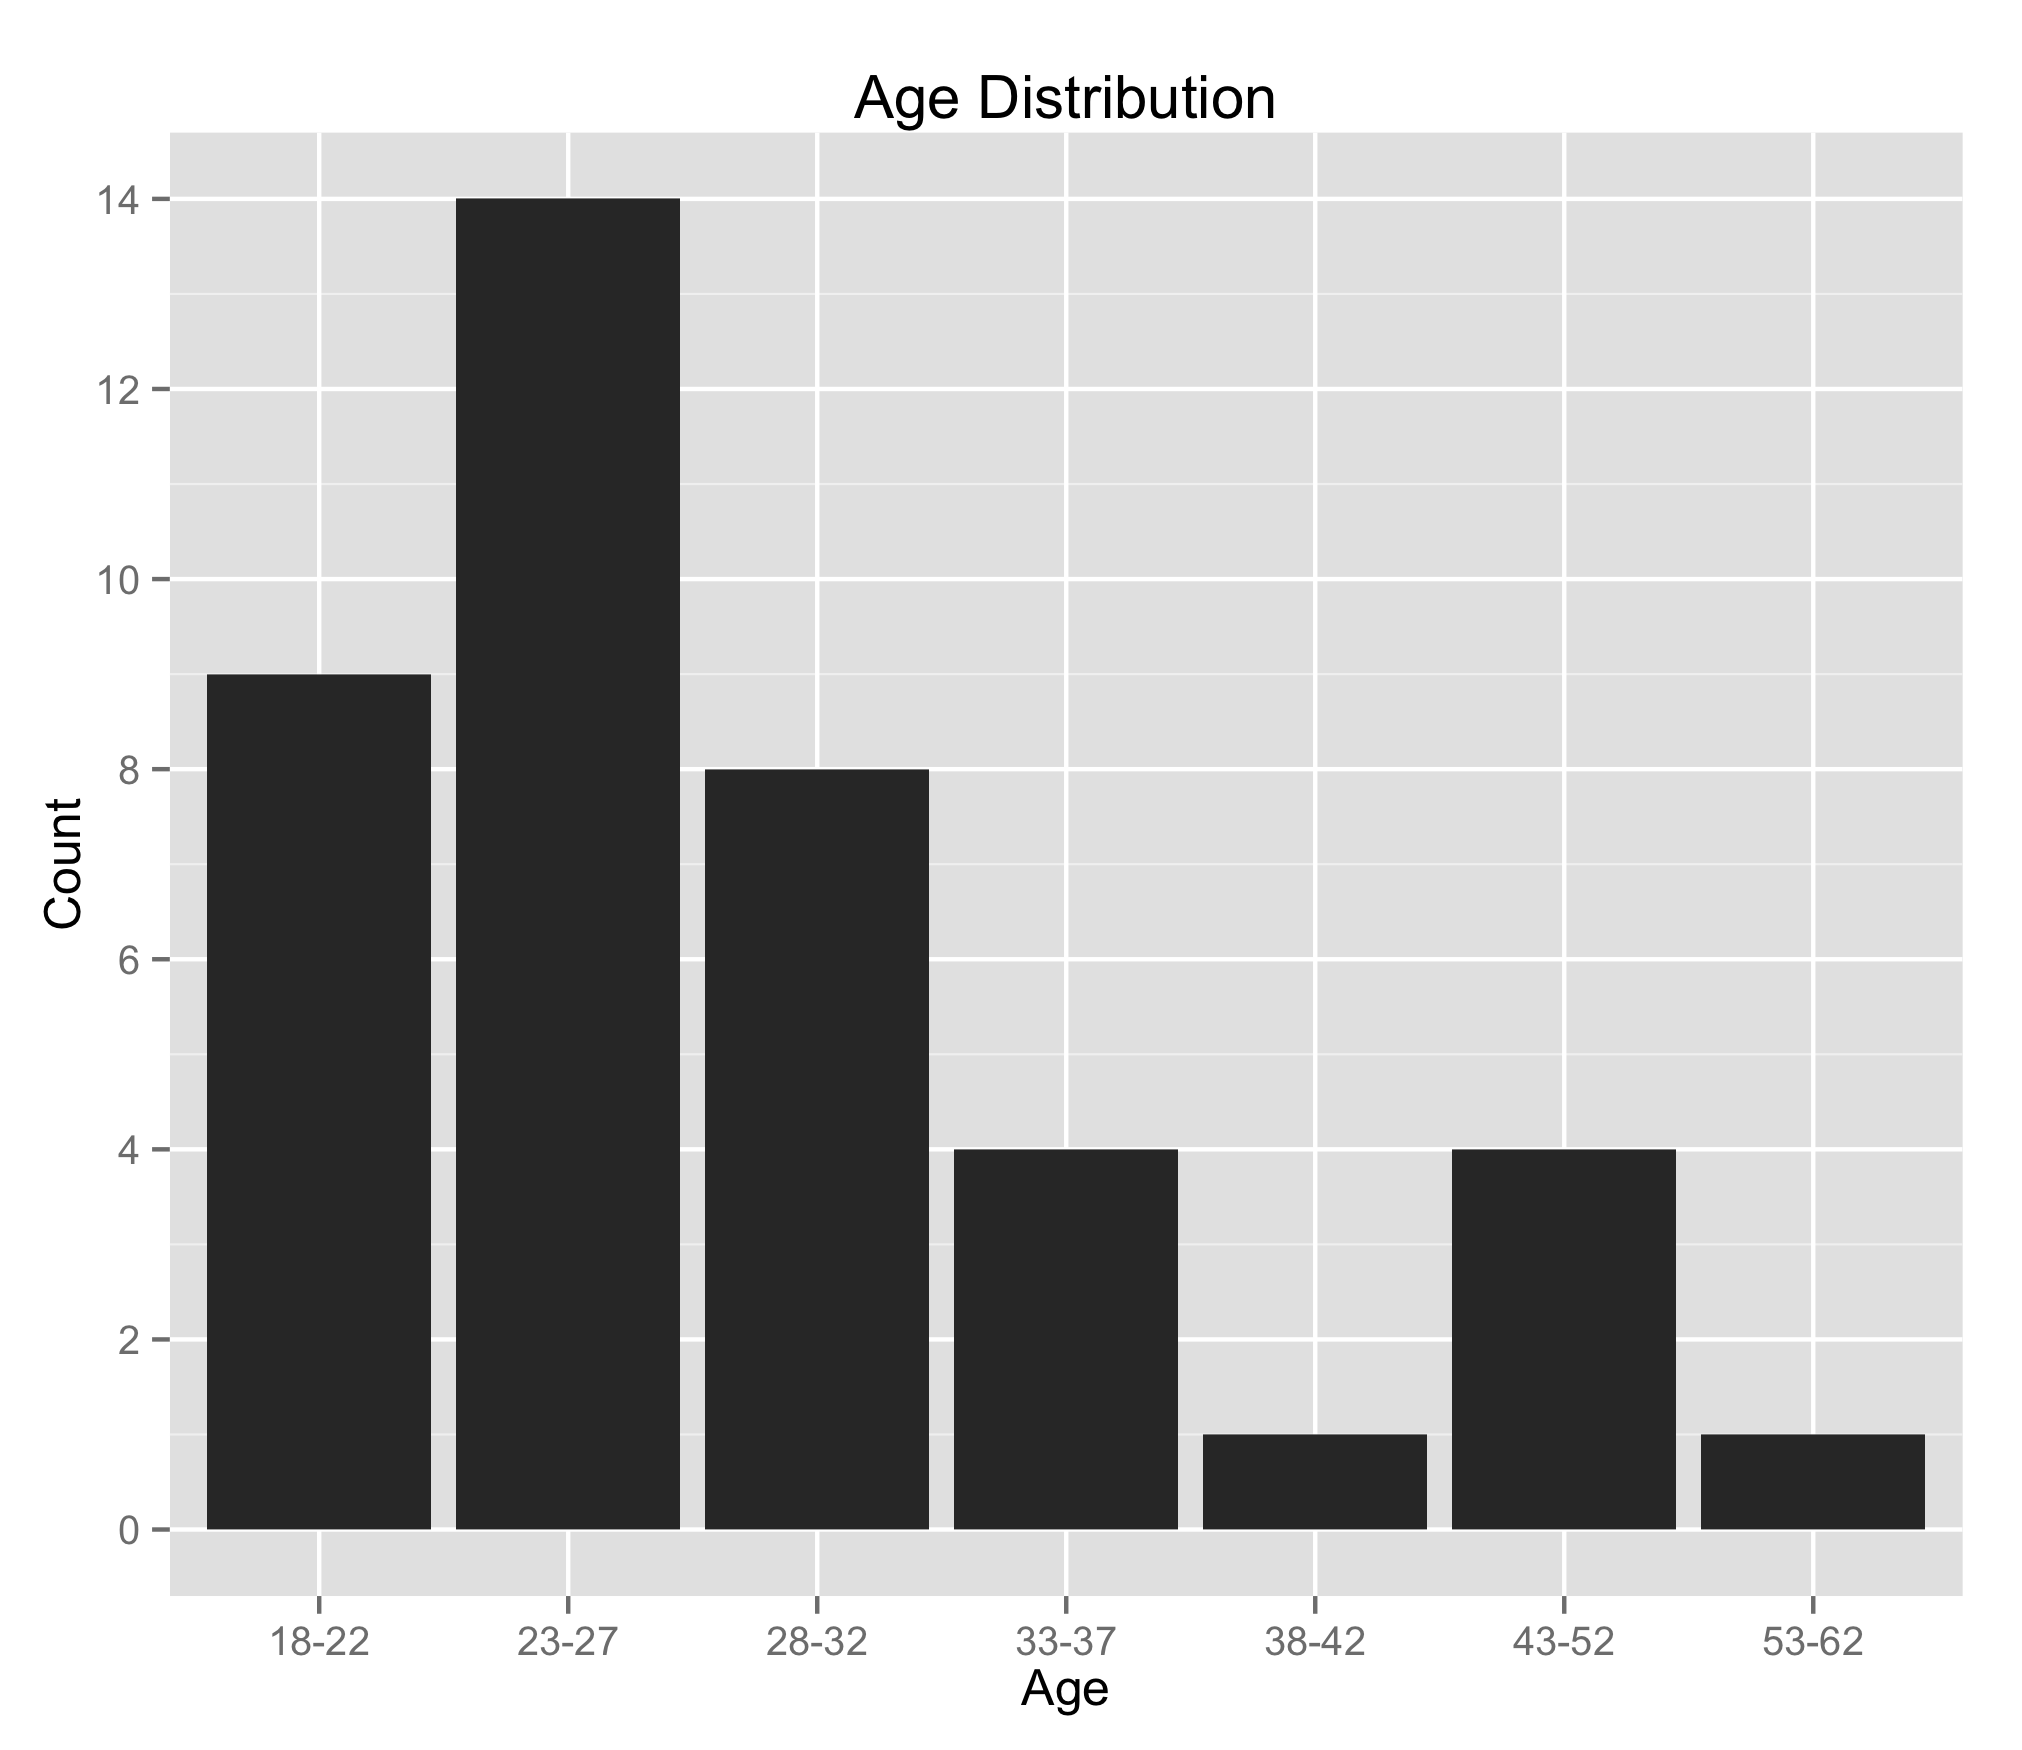
\includegraphics[width=1.0\linewidth]{graphs/age.png}
    \caption{Age Distribution}
    \label{agedistribution}
\end{subfigure}%
\begin{subfigure}{.5\textwidth}
    \centering
    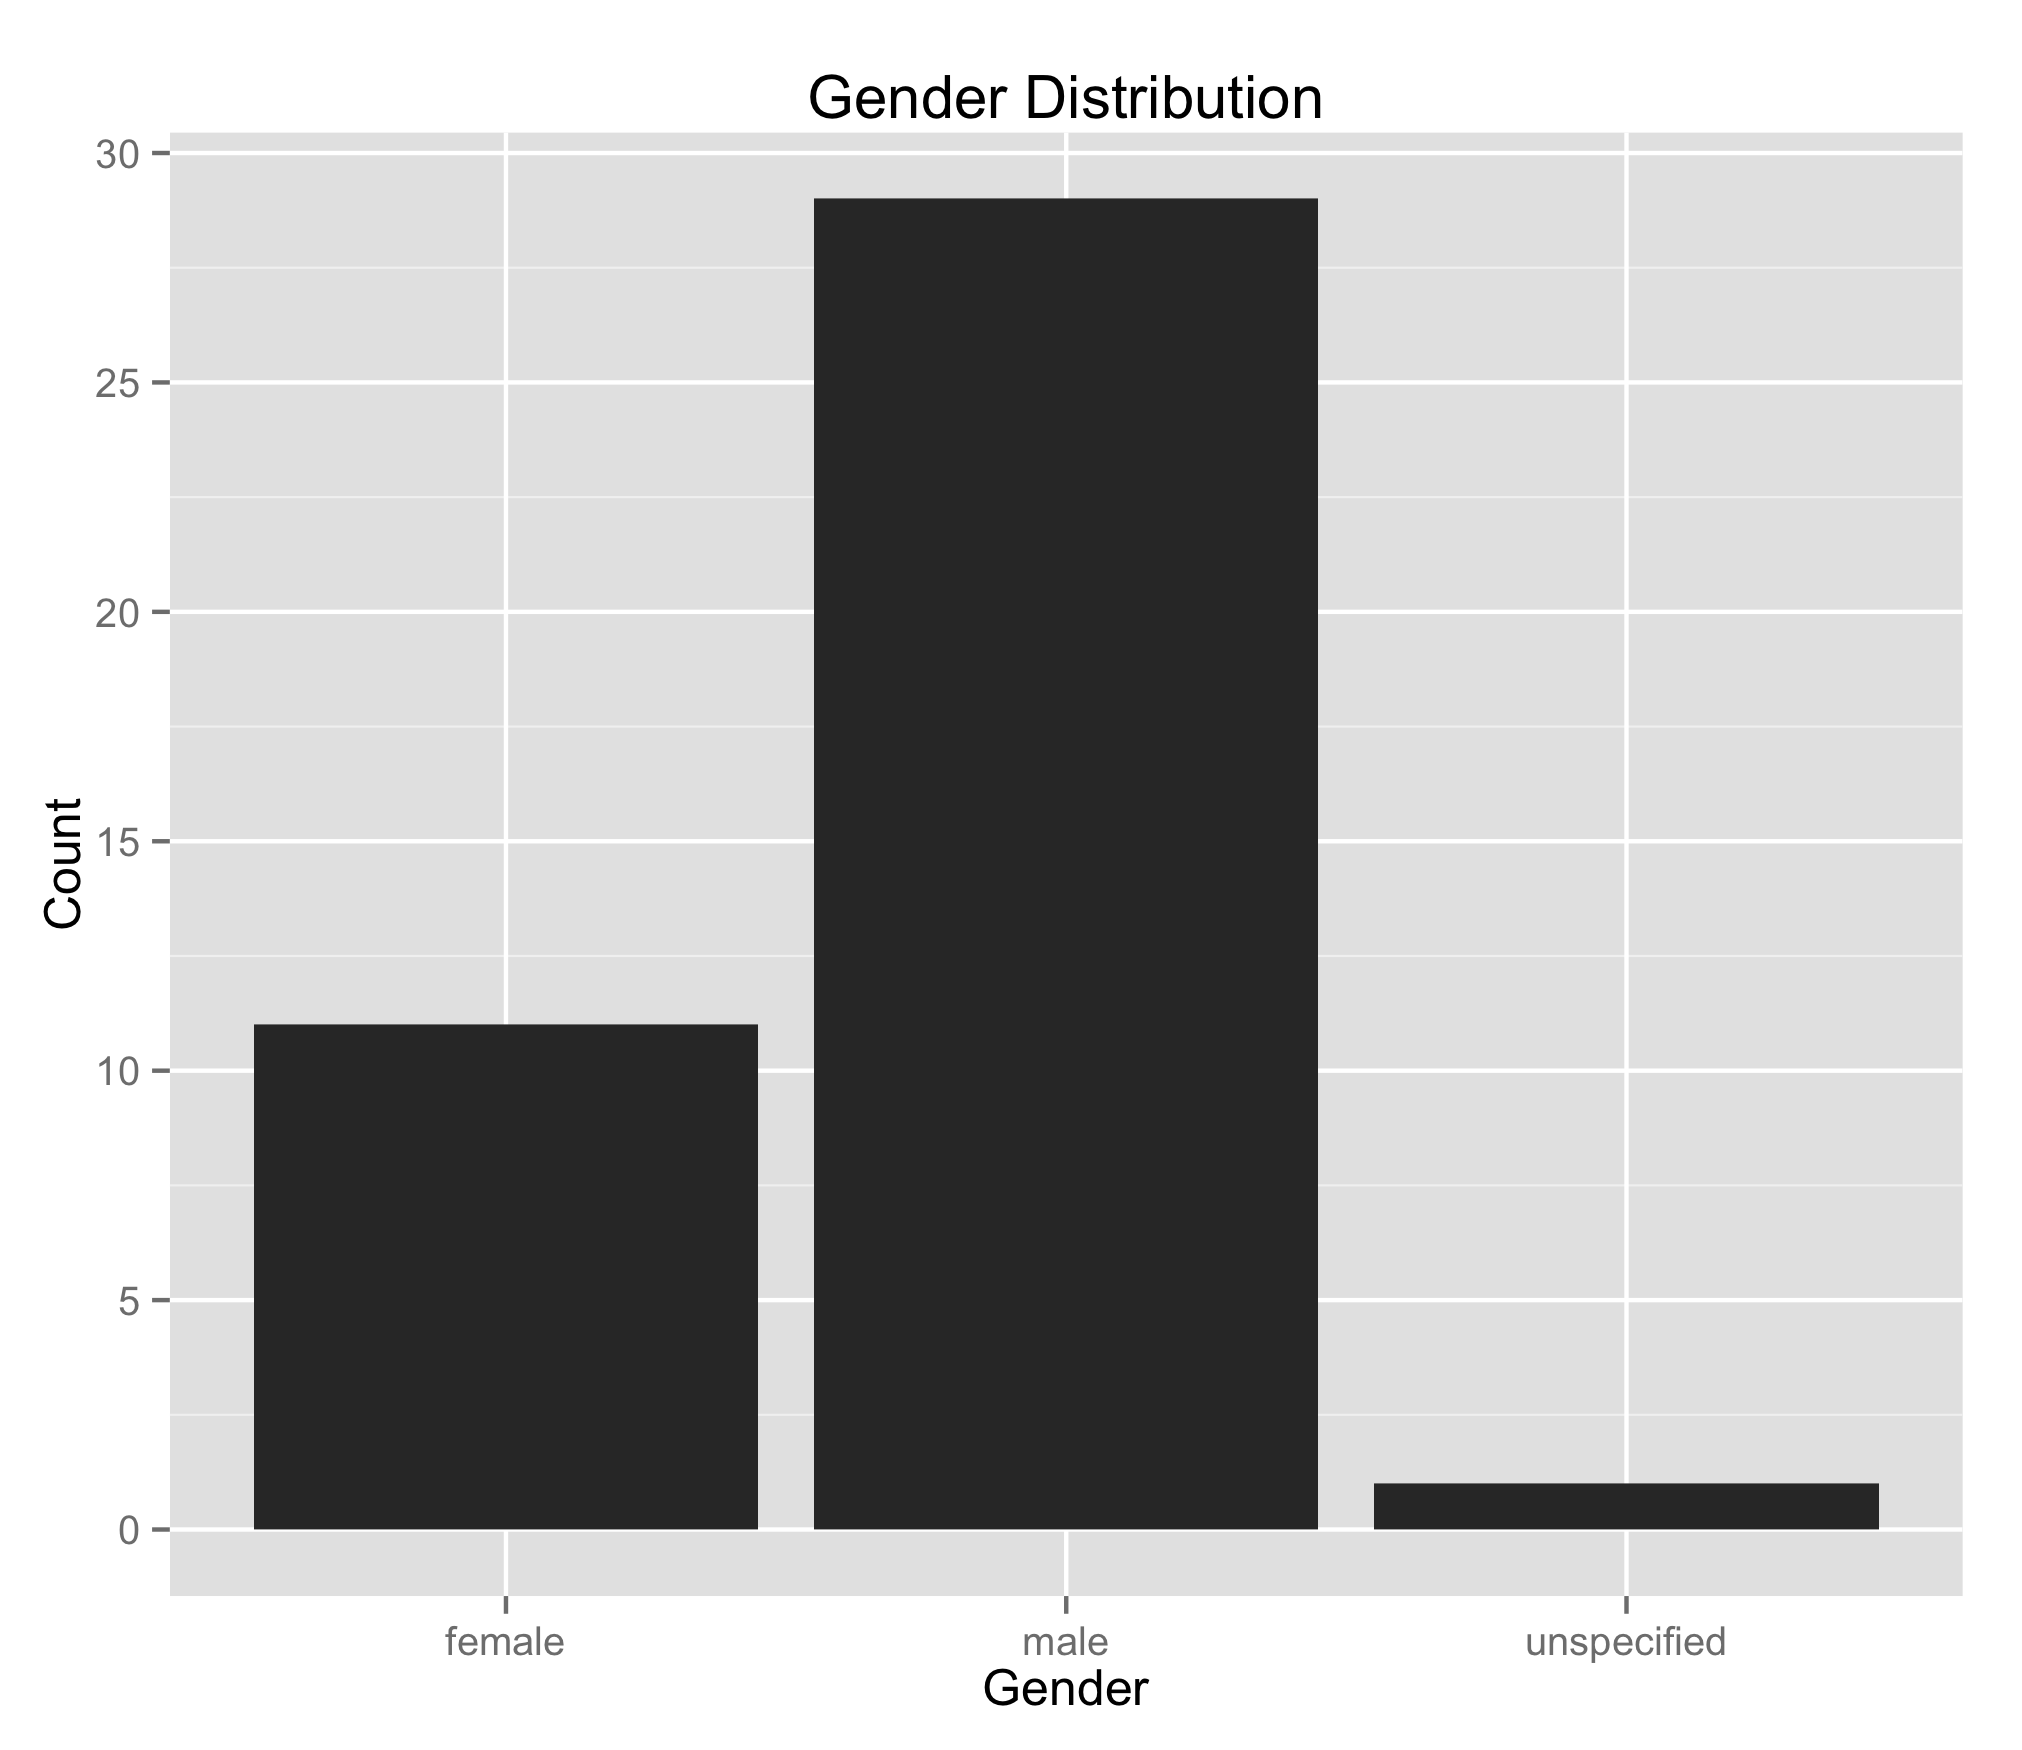
\includegraphics[width=1.0\linewidth]{graphs/gender.png}
    \caption{Gender Distribution}
    \label{genderdistribution}
\end{subfigure}
\caption{Basic Demographics}
\centering
\begin{subfigure}{.5\textwidth}
    \centering
    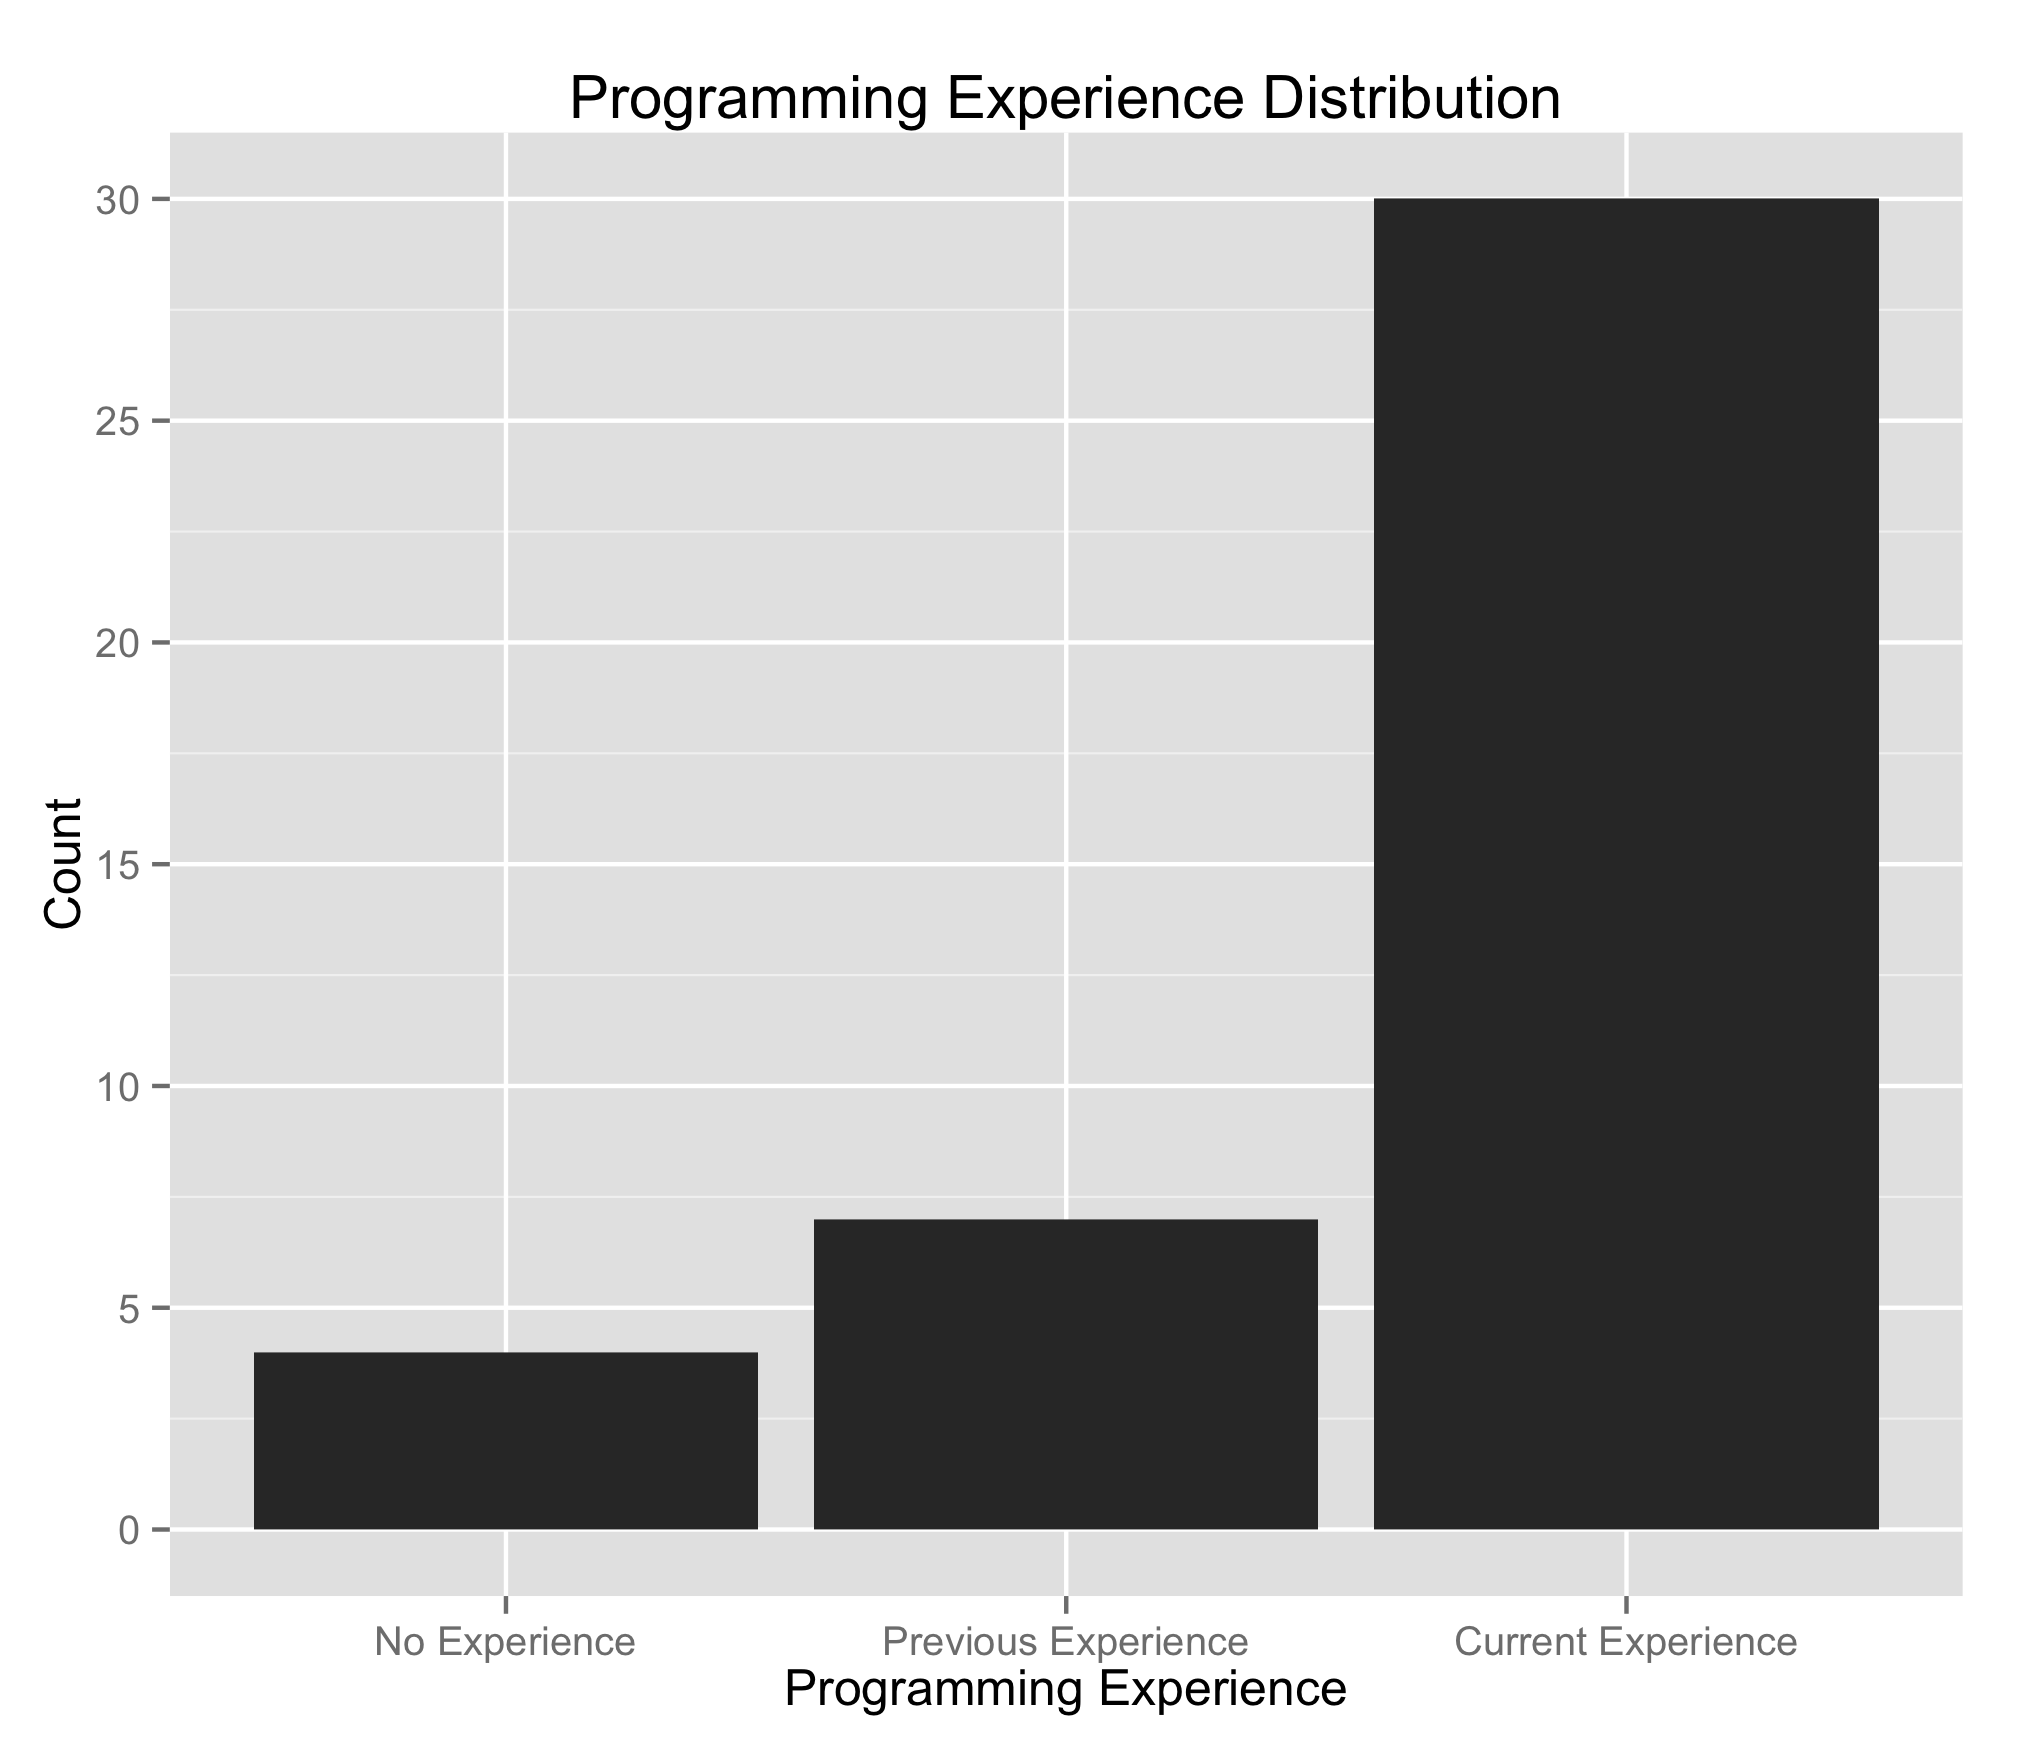
\includegraphics[width=1.0\linewidth]{graphs/programming.png}
    \caption{Programming Experience Distribution}
    \label{programmingdistribution}
\end{subfigure}%
\begin{subfigure}{.5\textwidth}
    \centering
    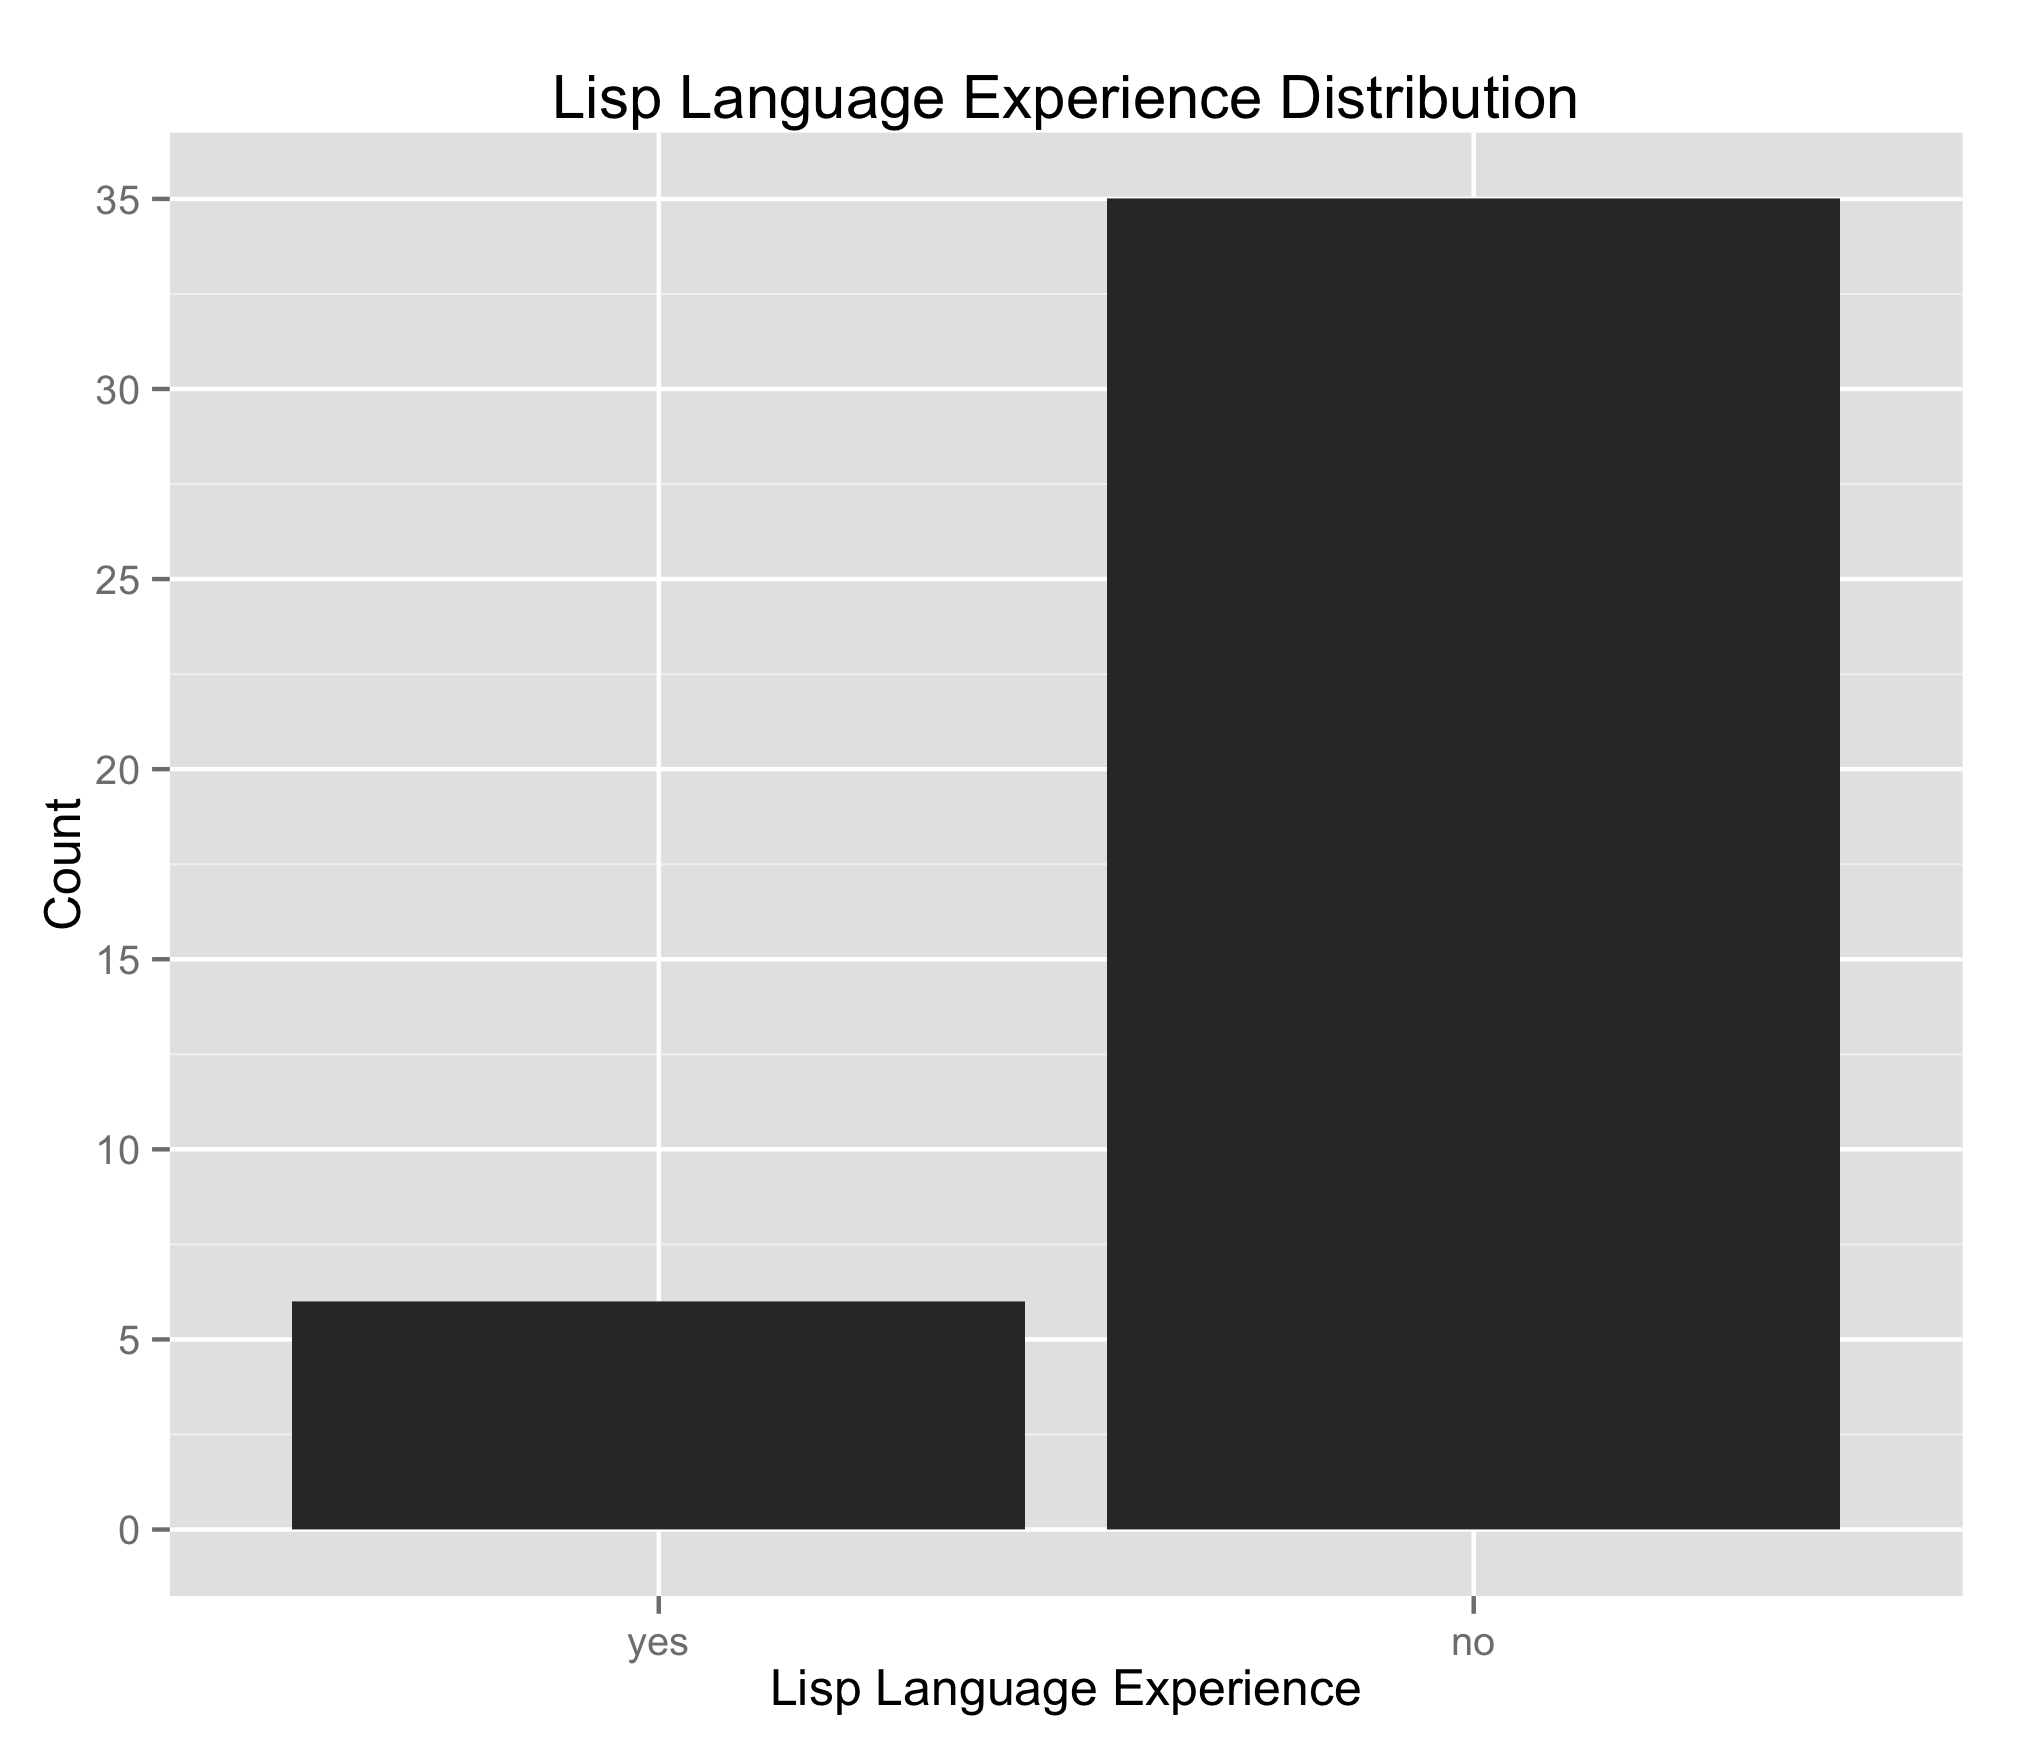
\includegraphics[width=1.0\linewidth]{graphs/lisp.png}
    \caption{Lisp Experience Distribution}
    \label{lispdistribution}
\end{subfigure}
\caption{Programming Demographics}
\end{figure}


\section{Method}
Two sets of visualisations were presented to an audience during a live coding performance and surveys were distributed. The performance was run as two ten minute improvised songs with each song demonstrating one of the two experimental visualisation conditions, either the didactic condition or the aesthetic condition. The experiment was run twice, with two separate participant groups, swapping the order in which the two sets of visualisations were presented to the audience.\\

The audience members completed a survey consisting of four sections over the course of the performance. These sections included a demographic information section, opinion of the first visualisation, opinion of the second visualisation and a section investigating the audience's overall opinion of the performance. The sections regarding the visualisations predominantly focussed on the enjoyment and understanding related to the visualisation while the final section focussed on eliciting potential improvements.\\

After explaining to the participants the structure of the experiment and allowing the participants to complete the initial demographic section of a survey, the live coder began the first performance utilising one of the two visualisations. Following this first set, the second section of the survey was conducted. A second set was then played using the alternative visualisation. Following this second set, the same survey questions were administered again, again asking the participants specifics about their enjoyment and understanding related to the specific visualisation demonstrated. A final survey question was then asked relating to their opinion regarding the whole performance and their suggested improvements.

\section{Participants}

A total of 41 participants took part in the study. Over the two performances, 19 participants observed the first performance and 22 participants observed the second performance. The demographic makeup between the two performances was very similar.\\

$66\%$ of the participants stated that they were male (see Figure \ref{genderdistribution}) and most participants were aged between 18 and 32 ($76\%$, see Figure \ref{agedistribution}). As the study was conducted within the Computer Science Department, a large proportion of the participants were experienced with programming with $90\%$ having current or previous experience with it (see Figure \ref{programmingdistribution}). Nevertheless, only $15\%$ of participants had previous experience with any of the Lisp style of languages (see Figure \ref{lispdistribution}).\\

Of the participants, $68\%$ stated that they listened to a large amount of music (see Figure \ref{musicdistribution}) though only about $15\%$ of participants stated that they played and instrument or sung regularly (see Figure \ref{instrumentdistribution}). Only $22\%$ of participants had seen a live coding performance before.\\


\begin{figure}[t]
\centering
\begin{subfigure}{.5\textwidth}
    \centering
    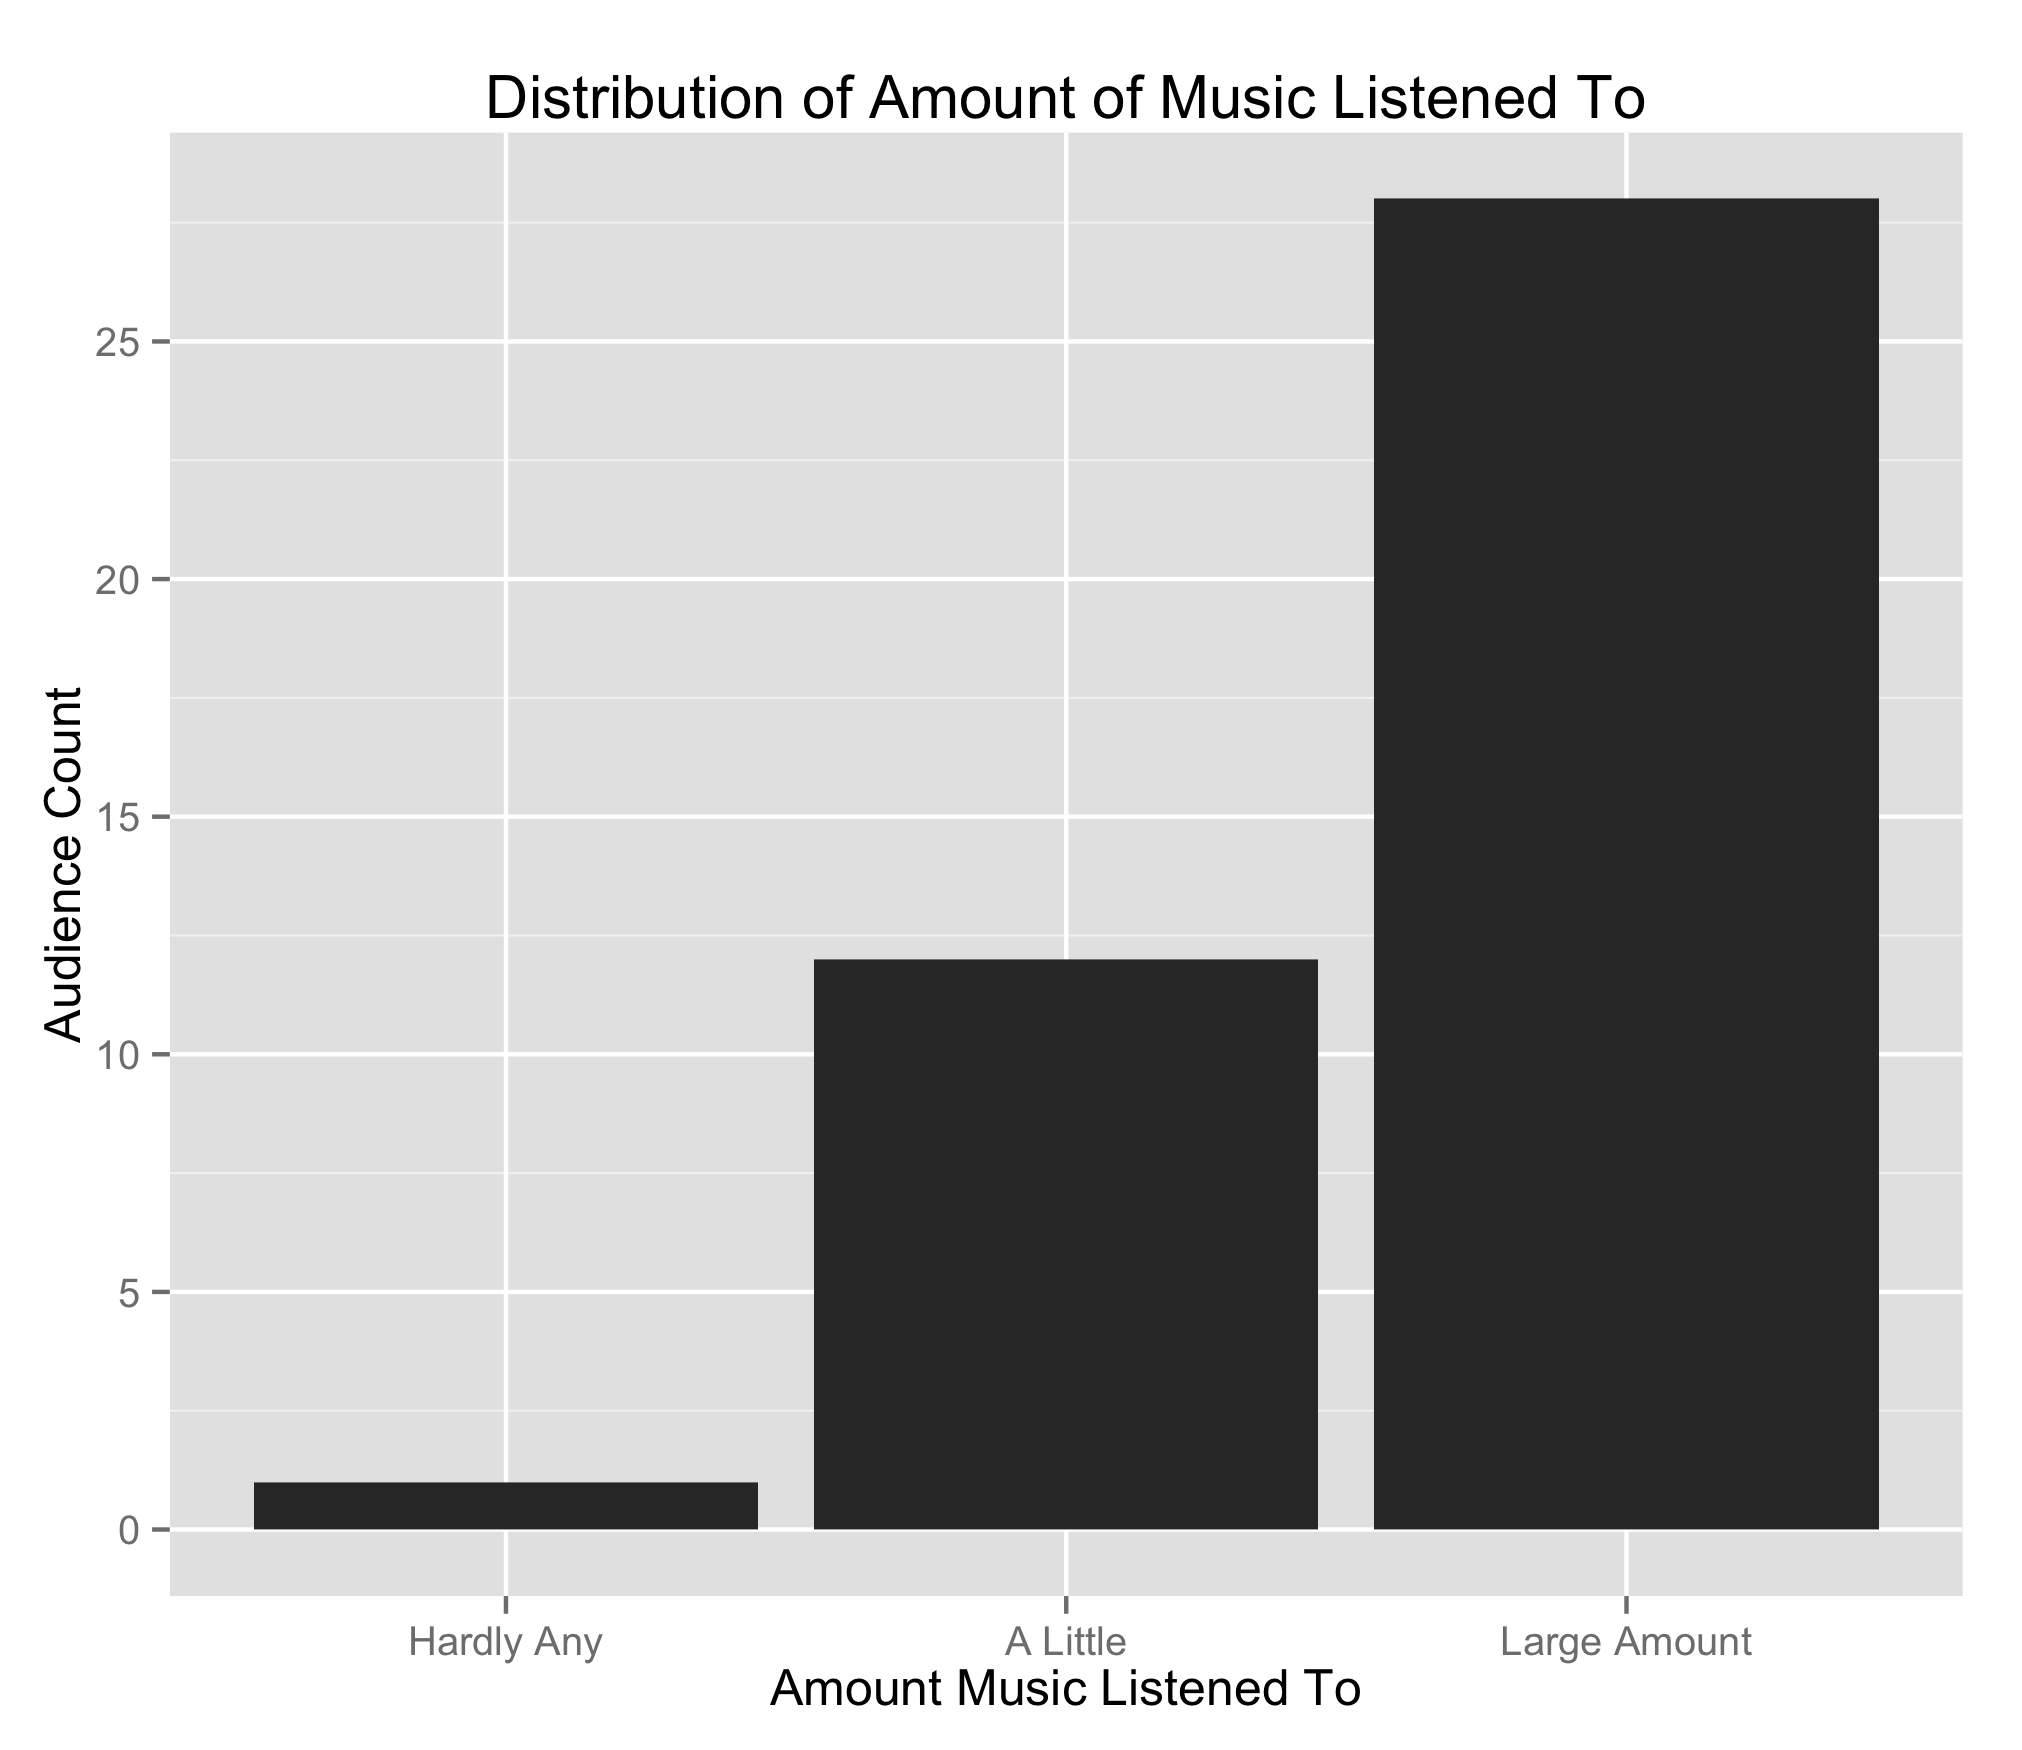
\includegraphics[width=1.0\linewidth]{graphs/music.png}
    \caption{Listen to Music Regularity Distribution}
    \label{musicdistribution}
\end{subfigure}%
\begin{subfigure}{.5\textwidth}
    \centering
    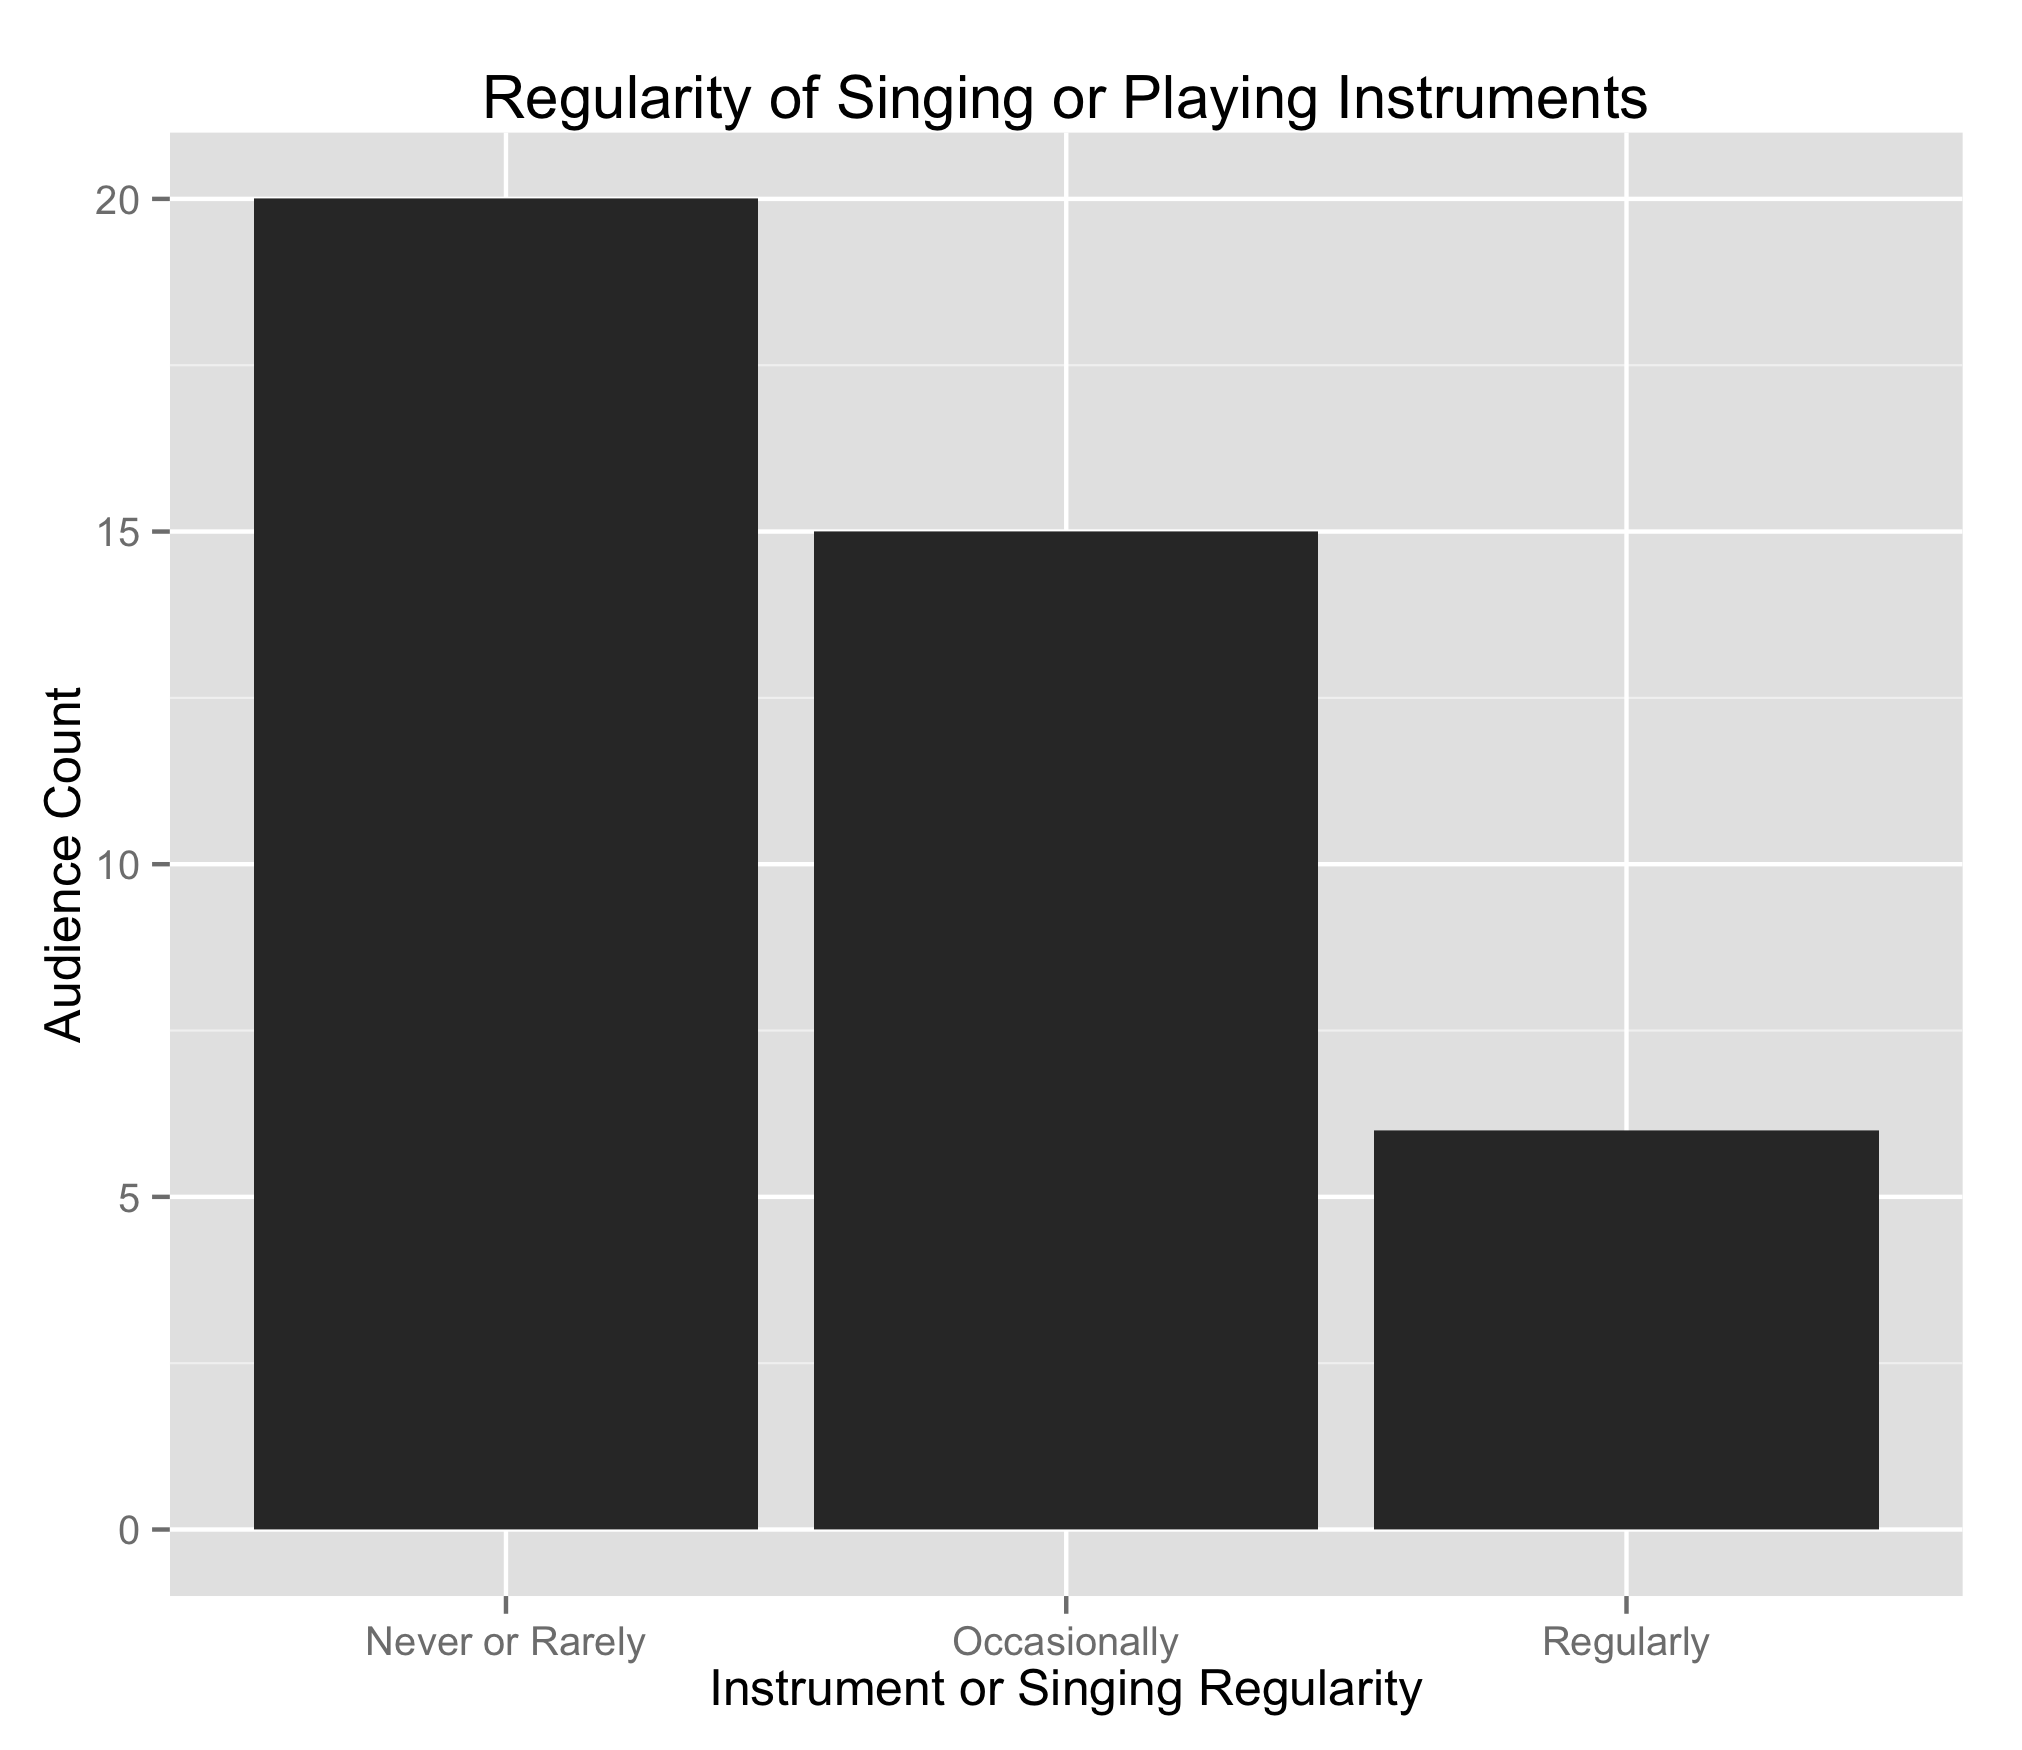
\includegraphics[width=1.0\linewidth]{graphs/instrument-regularity.png}
    \caption{Playing Instrument or Singing Regularity Distribution}
    \label{instrumentdistribution}
\end{subfigure}
\caption{Musical Demographics}
\end{figure}

\section{Results}

\subsection{Aesthetic vs Didactic Visualisation}

Understanding and enjoyment were evaluated against the didactic and aesthetic visualisations. Results and statistical analysis of the differences between the aesthetic and didactic conditions follows. Note that for the following statistical analysis a significance level of $0.05$ was used with the chi-squared test for independence.

\subsubsection{Understanding}
Overall, $37\%$ participants stated specifically that the didactic visualisations helped them to understand the code, whereas $12\%$ participants stated that the aesthetic visualisations assisted in understanding the code.\\

$H_0$: There is no difference between the aesthetic visualisations and didactic visualisations in terms of understanding.\\
$H_1$: There is a difference between the two visualisations in terms of understanding.\\

A significant difference between the visualisations effect on understanding was found ($\chi^2=7.1986,df=2,p=0.02734$).

\subsubsection{Enjoyment}
Overall, for both visualisations, a large proportion ($> 50\%$) of the participants stated that the visualisations helped their enjoyment of the performance. Of the participants, $76\%$ stated that the aesthetic visualisations helped their enjoyment compared to $56\%$ participants that stated the didactic visualisations helped their enjoyment.\\

There was indication that any decreases in enjoyment may have been postponed when shown the aesthetic visualisation and that there was overall an increasing enjoyment during the middle of the performance when this visualisation was shown. See Figure \ref{aestheticenjoymentchange} and Figure \ref{didacticenjoymentchange} for the distribution of changes to enjoyment between the aesthetic and didactic visualisations.\\

$H_0$: There is no difference between the aesthetic visualisations and didactic visualisations in terms of enjoyment.\\
$H_1$: There is a difference between the two visualisations in terms of enjoyment.\\

No significant difference between the two visualisations effect on enjoyment was found ($\chi^2=3.7733,df=2,p=0.1516$).

\begin{figure}[t]
\centering
\begin{subfigure}{.5\textwidth}
    \centering
    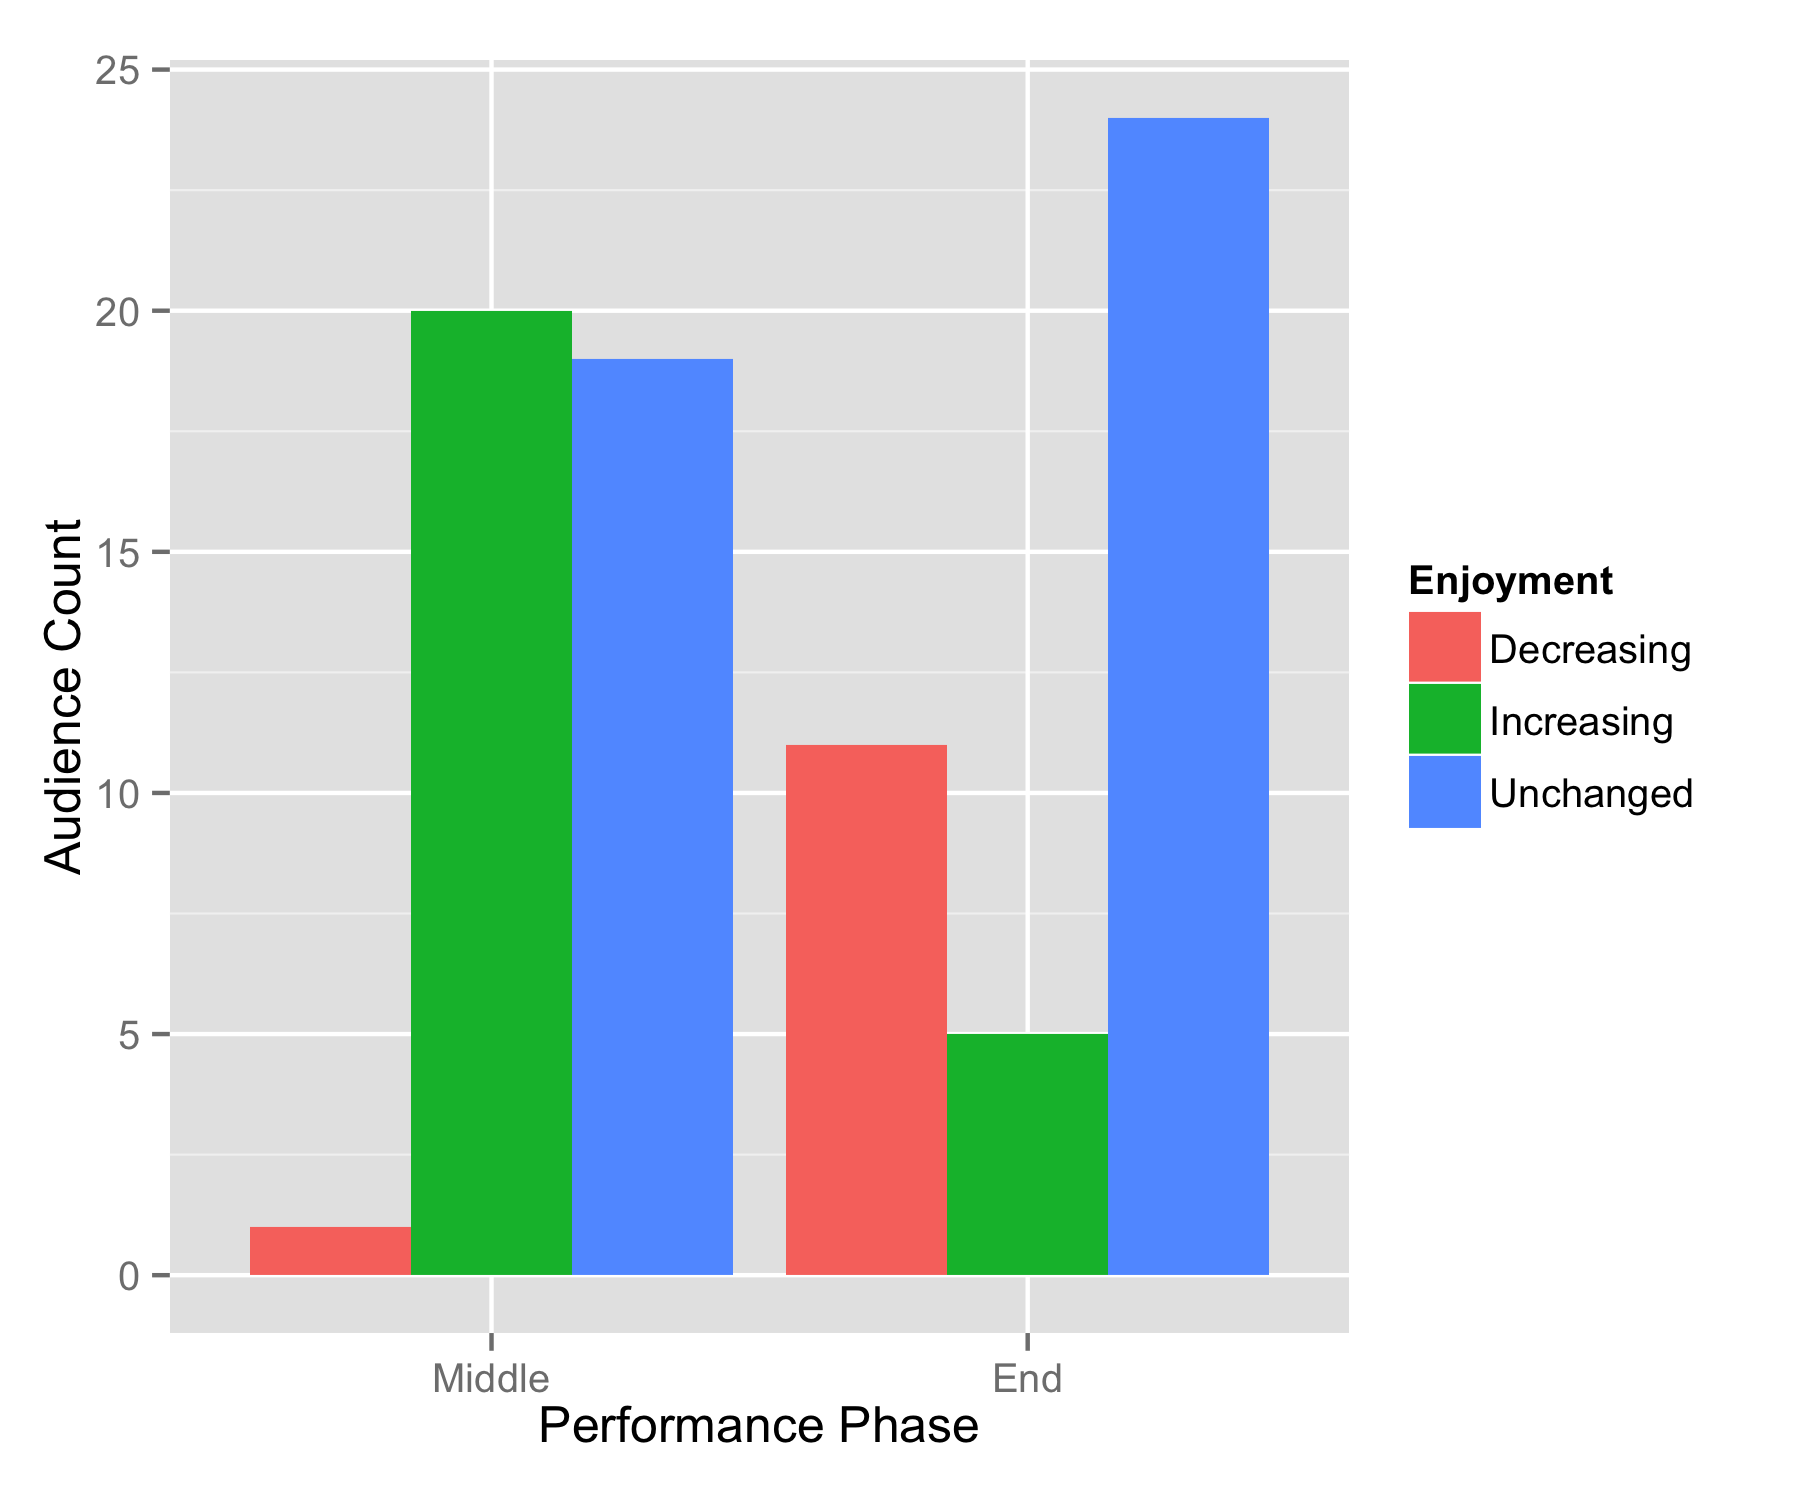
\includegraphics[width=1.0\linewidth]{graphs/enjoyment-change-aesthetic.png}
    \caption{Aesthetic Visualisation}
    \label{aestheticenjoymentchange}
\end{subfigure}%
\begin{subfigure}{.5\textwidth}
    \centering
    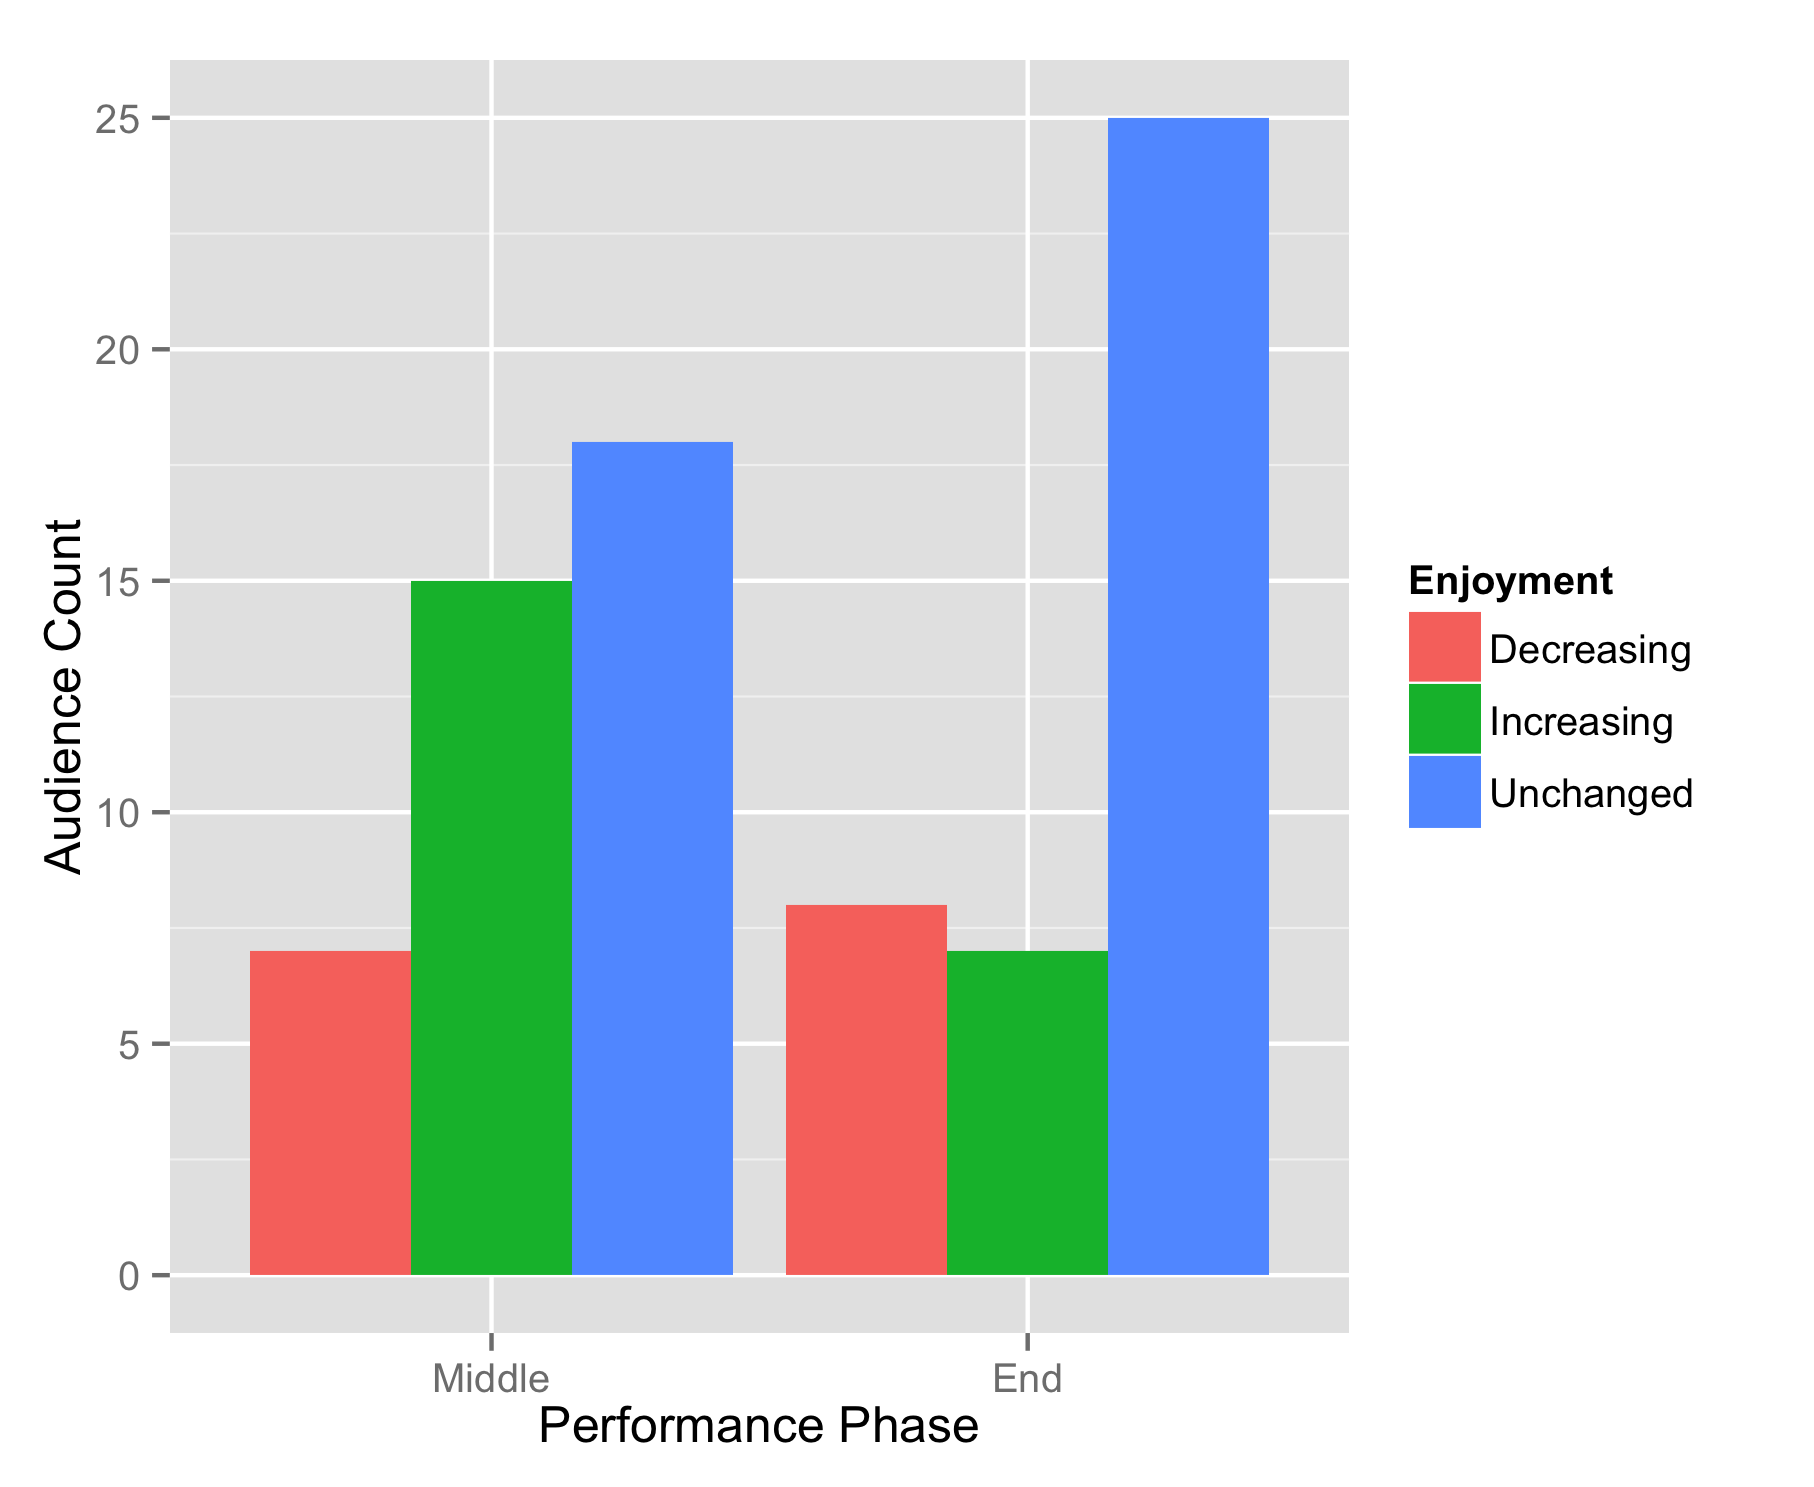
\includegraphics[width=1.0\linewidth]{graphs/enjoyment-change-didactic.png}
    \caption{Didactic Visualisation}
    \label{didacticenjoymentchange}
\end{subfigure}
\caption{Change of enjoyment through specific phases of the performance for aesthetic and didactic visualisations}
\end{figure}

\subsubsection{Liveness}

Participants were asked to discuss how each visualisation influenced or impacted the liveness of the performance. Concepts discussed included the positive and negative aspects of the didactic visualisations, the positive and negative aspects of the aesthetic visualisations, source code discussion and statements indicating an understanding between the visuals and the source code. A summary of the references and coverage of these concepts is available in Table \ref{tab:livenesscoverage}. The references column indicates the number of times the concept was mentioned and the coverage indicates the total amount of discussion of the concept.

\begin{table}
\caption {Liveness Concept Coverage from Audience Feedback} \label{tab:livenesscoverage} 
\begin{center}
\begin{tabular}{ l | c c }

Concept&References&Coverage\\
\hline
Negative Didactic Aspects&26&17\%\\
Positive Didactic Aspects&19&12\%\\
Negative Aesthetic Aspects&21&11\%\\
Positive Aesthetic Aspects&14&8\%\\
Source Code&40&28\%\\
Demonstrating Understanding&6&5\%\\
\end{tabular}
\end{center}
\end{table}

\subsection{Improvements}

The audience was asked what improvements to the visualisations they would like to see. 40\% of the audience suggested improvements that indicate a desire to see more relationship between the visualisations and the music, with suggestions such as matching the visualisations to musical rythms or pitch.\\

Other suggestions included increasing the readability of source code,  increasing uniformity between the visualisations and the use of images to assist with the understanding of high level concepts.

\section{Discussion}

Overall enjoyment of the visualisations was high. This was the case for both the aesthetic and didactic visualisations. However, it is interesting to note that enjoyment of the aesthetic visualisation was higher and generally increased during the earlier stages of the performances suggesting that the aesthetic visualisations held the audience's attention for longer (as shown in Figure \ref{aestheticenjoymentchange}). The didactic visualisation on the other hand had a more constant decrease in enjoyment. The audience improvements offer some insight into this suggesting that the visualisations were competing with the projected code.\\

Although the results surrounding the understanding afforded by the visualisations are unsurprising with the didactic visualisations having a clear educational benefit over the aesthetic visualisations, this will provide a baseline for future visualisations. Some improvements suggested by the audience will be examined in more detail and potentially implemeneted. For example, a number of participants stated that the didactic visualisations were distracting, too abrupt or took away from the code in other ways. On the other hand, some said that the didactic visualisations gave the performance a sense of being 'too polished'. The general consensus, however, was that the visualisation should either better reflect the code, better reflect the music or have more variety.\\

The overall reponse indicates that there is much potential to improve the examined visualisations, developing both the aesthetic aspects of the visualisations in addition to the educational aspects. Future visualisations will focus on taking advantage of the prolonged attention afforded by the aesthetic visualisations and combine it with the more educational aspects of the didactic visualisations demonstrated within this experiement. With these results there is some progress towards an effective interactive programming environment visualisation.

\bibliography{references}

\newpage
\section*{Appendix A}

\begin{figure}[H]
\centering
\begin{subfigure}{.5\textwidth}
    \centering
    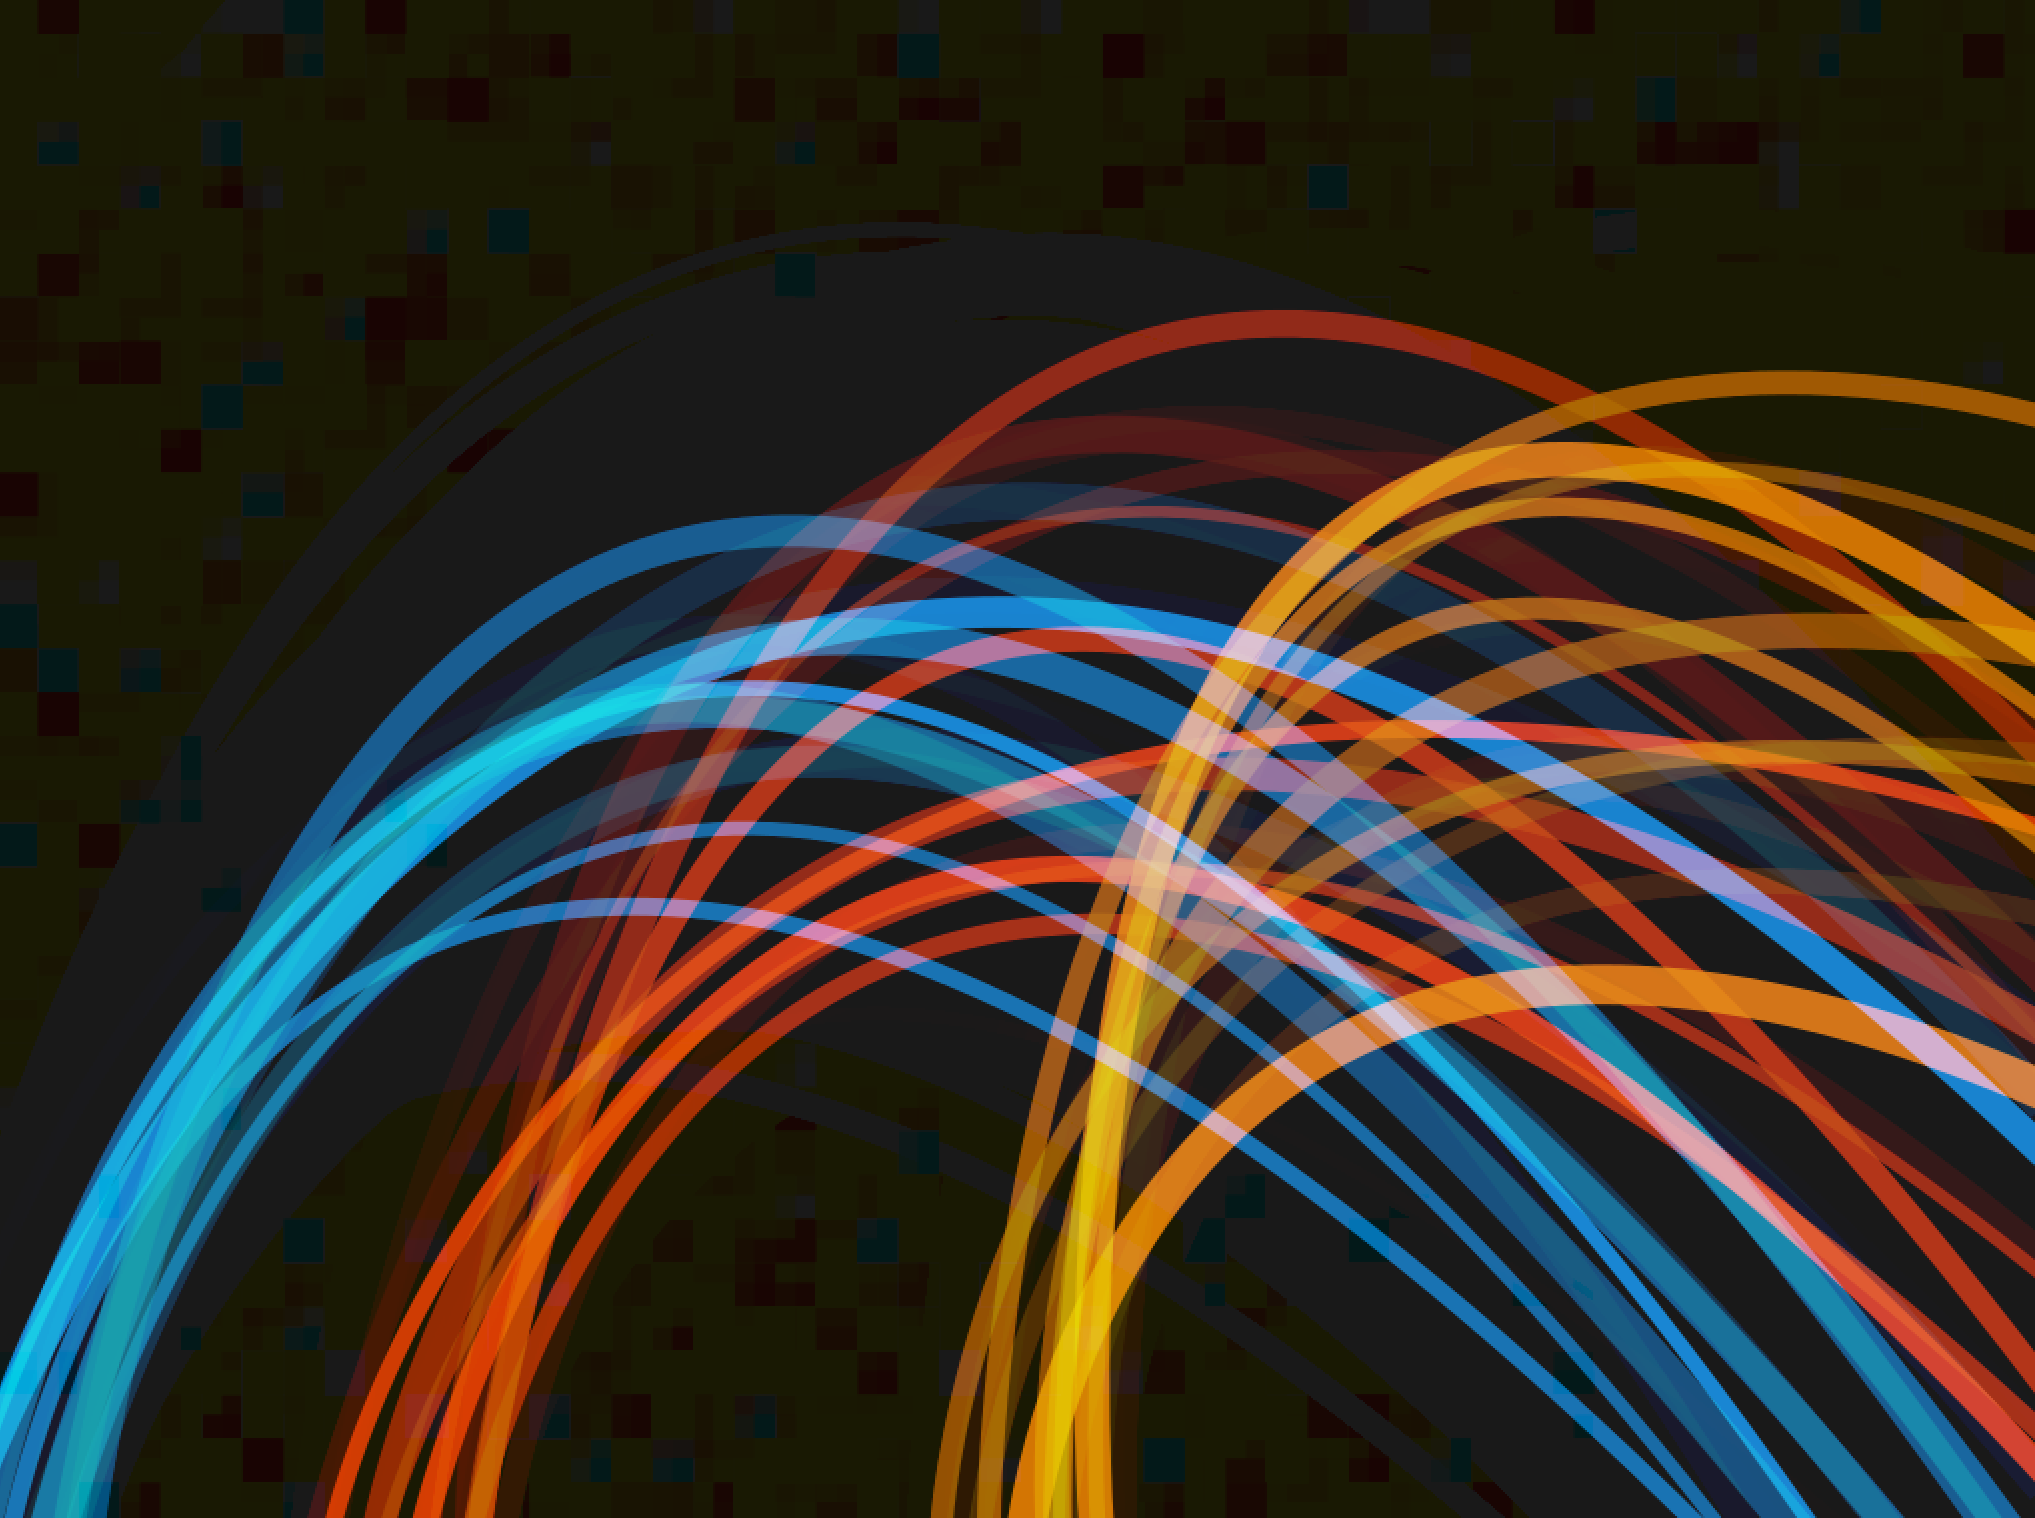
\includegraphics[width=0.9\linewidth]{aesthetic-vis.png}
    \caption{Aesthetic Visualisation}
    \label{avis}
\end{subfigure}%
\begin{subfigure}{.5\textwidth}
    \centering
    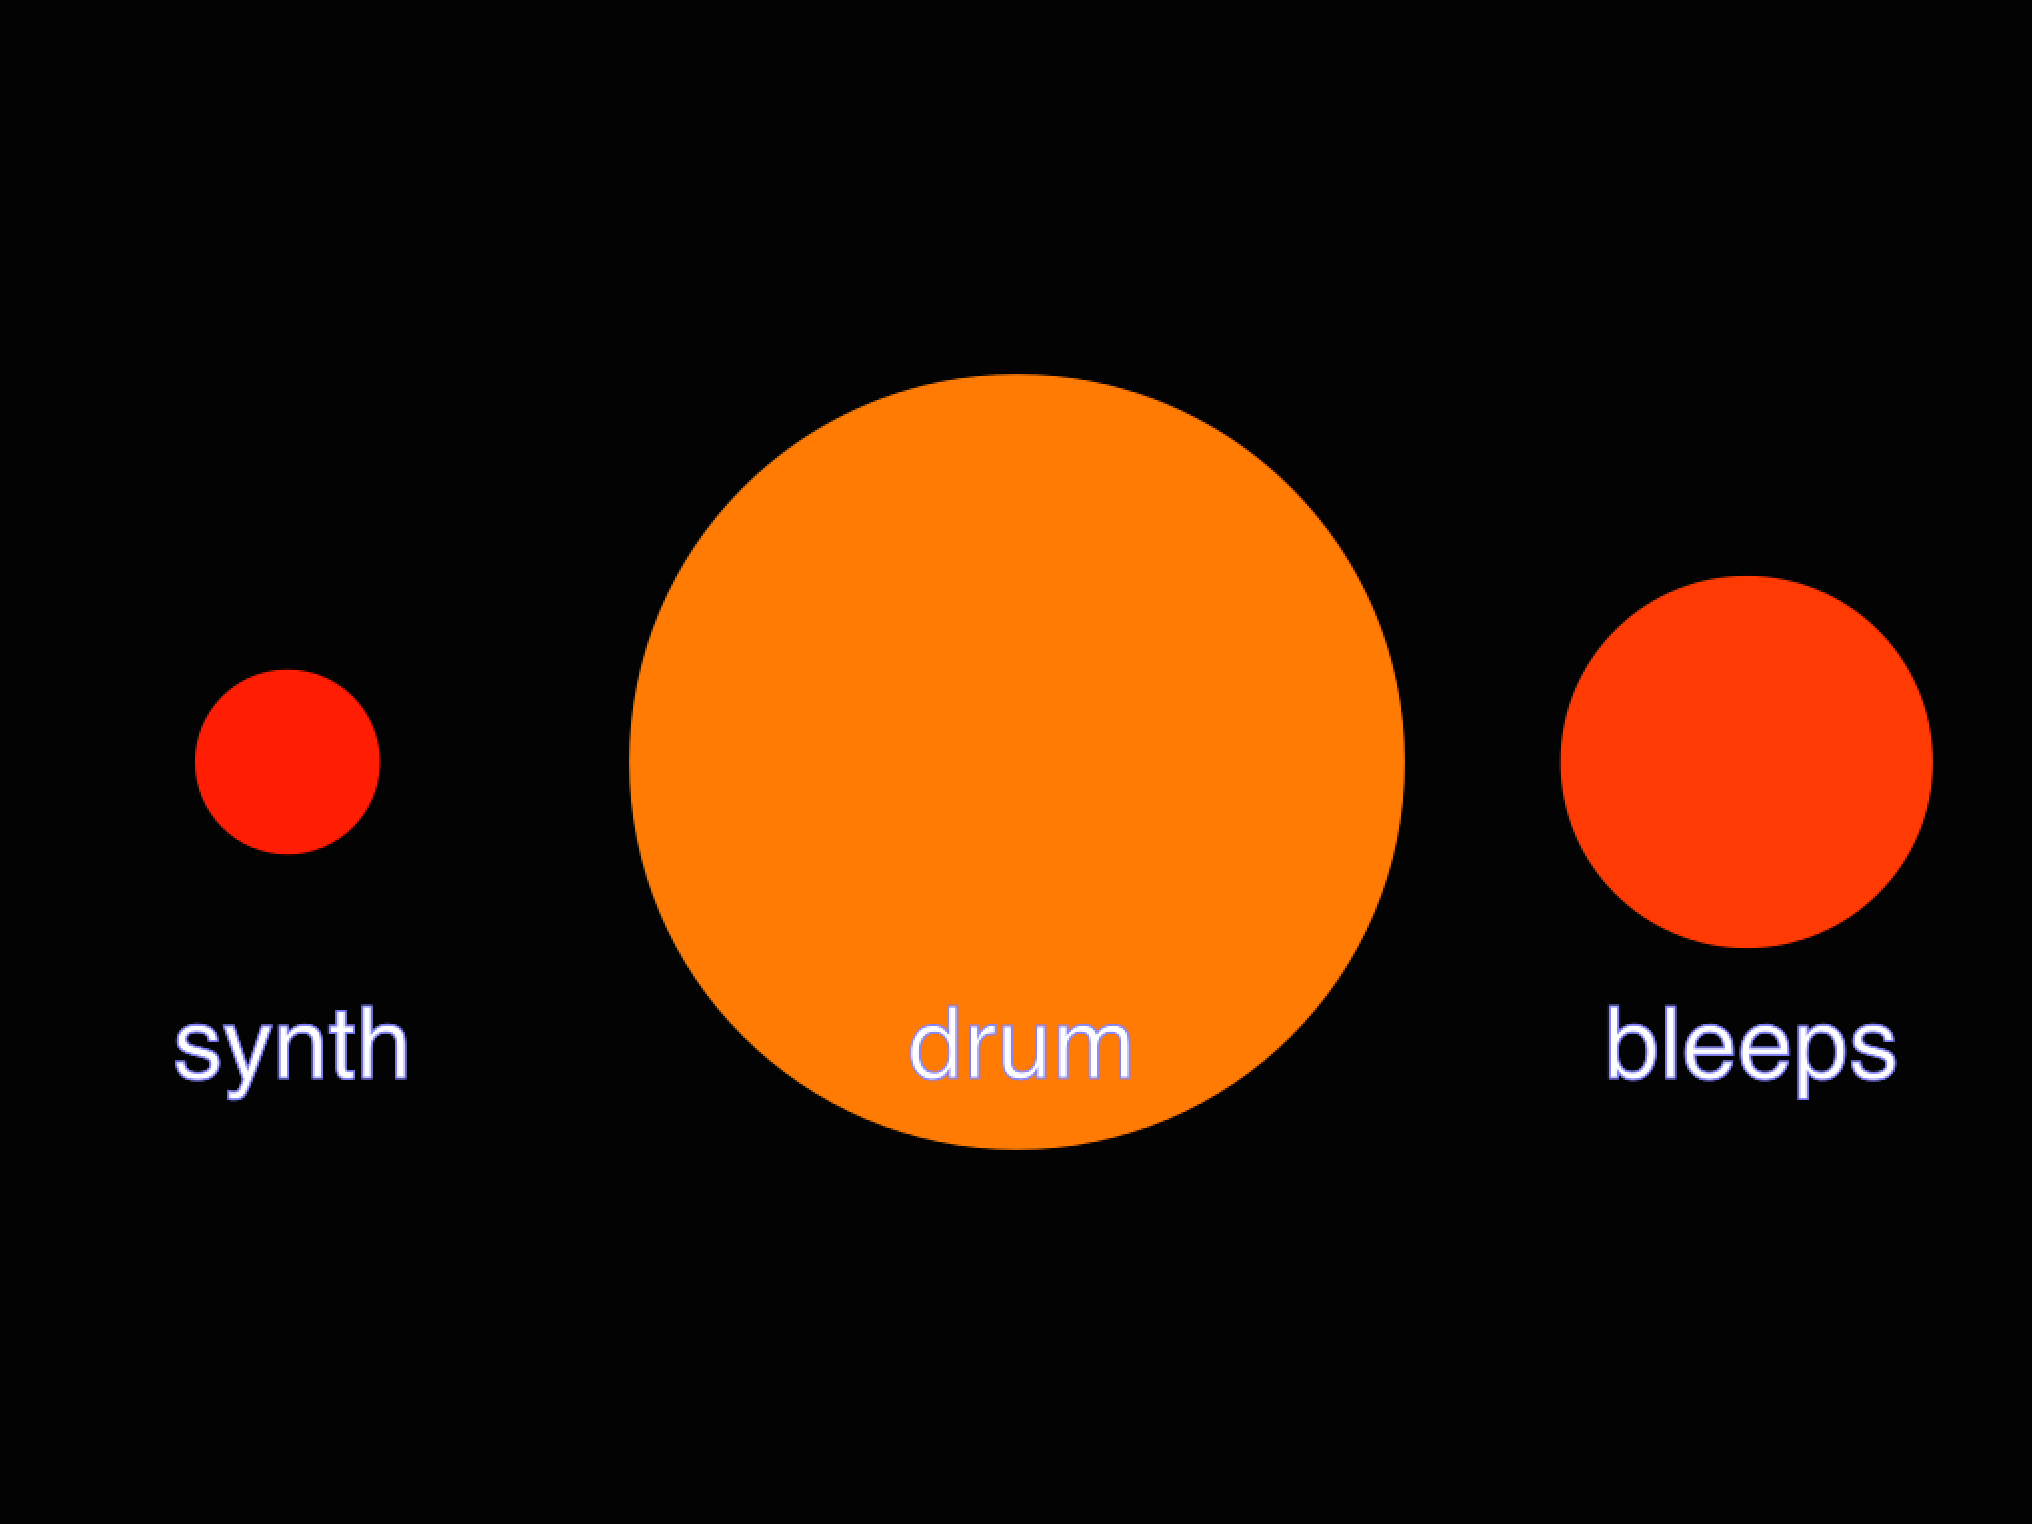
\includegraphics[width=0.9\linewidth]{didactic-vis.png}
    \caption{Didactic Visualisation}
    \label{dvis}
\end{subfigure}
\caption{Visualisation Examples}
\end{figure}


\end{document}